%\documentclass[12pt,a4paper,oneside]{book}
%\documentclass[12pt,a4paper,twoside]{book}
\documentclass[11pt,a4paper,twoside,titlepage,openany]{book}

%\usepackage[outer=1.5cm,inner=2.5cm,top=2cm,bottom=2cm]{geometry}
%\usepackage[outer=3cm,inner=3cm,top=4cm,bottom=3cm]{geometry}
\usepackage[outer=3.5cm,inner=3.5cm,bottom=4cm]{geometry}

\usepackage[english]{babel}

\usepackage[hidelinks,breaklinks]{hyperref}  % added

\usepackage{amsthm}
\usepackage{graphicx}
\usepackage{amssymb}
%\usepackage{natbib}
\usepackage[numbers]{natbib}
\usepackage{rotating}
\usepackage{multirow}
\usepackage{enumerate}
\usepackage{color}
\usepackage{comment}

% added
\usepackage{listings}
 \lstset{basicstyle=\footnotesize\ttfamily,frame=lines}
 %\lstset{basicstyle=\footnotesize,keywordstyle=\color{blue},}
 %\lstset{basicstyle=\small\ttfamily,frame=single}
 \AtBeginDocument{\DeclareCaptionSubType{lstlisting}} % must stay between listings and subcaption
\usepackage{subcaption}
\usepackage[super]{nth}
%\usepackage[xindy,toc]{glossaries}
\usepackage[nottoc,chapter]{tocbibind} % ToC item for Bibliography at chapter level [no ToC item for ToC]
\usepackage[boxed,algochapter,vlined]{algorithm2e}
\usepackage{indentfirst}  % Indent first line of first paragraph of chapters/sections/...
\usepackage[inline]{enumitem}
 \newlist{inlineenum}{enumerate*}{1}
 \setlist[inlineenum]{label=\textit{\roman*})}
\usepackage{tikz}
 \usetikzlibrary{positioning}
 \usetikzlibrary{calc}
\renewcommand{\bottomfraction}{0.6}  %
\renewcommand{\topfraction}{0.75}    %  Fit more figures in text pages
\newcommand{\mono}[1]{{\footnotesize \ttfamily #1}}

% TODO notes
\usepackage{xcolor}  % would anyway be imported by todonotes
\colorlet{lightorange}{orange!40}  % 40% orange, 60% white
\usepackage[colorinlistoftodos,linecolor=orange,backgroundcolor=lightorange]{todonotes}
%% Usage: \todo{margin note} or \todo[inline]{note in a full-width box}

\usepackage{csvsimple}  % read csv to table
\usepackage{booktabs}   % table styling

% Glossary
\usepackage[xindy,toc]{glossaries}  % nomain allows for 
%\loadglsentries[main]{SDN-glossary}
\newacronym{SDN}{SDN}{software defined networking}
\newacronym{ICN}{ICN}{information-centric networking}
\newacronym{NDN}{NDN}{named data networking}
\newacronym{NFV}{NFV}{network function virtualization}
\newacronym{CCN}{CCN}{content-centric networking}
% specific to ICN
\newacronym{FIB}{FIB}{forwarding information base}
\newacronym{PIT}{PIT}{pending interest table}
\newacronym{CS}{CS}{content store}
% other
\newacronym{Mpps}{Mpps}{millions packets per second}
\newacronym{NUMA}{NUMA}{non-uniform memory access}
\glsunset{NUMA}  % prevents expansion at first occurrence
\newacronym{DMA}{DMA}{direct memory access} \glsunset{DMA}
\newacronym{NIC}{NIC}{network interface card} \glsunset{NIC}
\newacronym{CRC}{CRC}{cyclic redundancy check} \glsunset{CRC}
\newacronym{PDU}{PDU}{protocol data unit}
\newacronym{SDU}{SDU}{service data unit}

\makeglossaries

% for allowing forced newlines inside table header cells
% from http://tex.stackexchange.com/a/19678/25479
\newcommand{\specialcell}[2][c]{%
  \begin{tabular}[#1]{@{}c@{}}#2\end{tabular}}

\bibliographystyle{alpha}
%\bibliographystyle{plain}
%\bibliographystyle{plainnat}  % allows \citeauthor but still uses numbering with [numbers]
%\bibliographystyle{unsrtnat}  % allows \citeauthor but still uses numbering with [numbers]
%\usepackage[all]{nowidow}  % Tries to prevent widow lines


% vvv  Acknowledgemts in cima  vvv
\makeatletter
\newcommand\ackname{Acknowledgements}
\newenvironment{acknowledgements}{
  \newpage
  \thispagestyle{empty}
  \null\vfil
  \@beginparpenalty\@lowpenalty
  \begin{center}
    % \bfseries \ackname  % tolto da me
    \@endparpenalty\@M
  \end{center}}
{\par\vfil\null\endtitlepage}
\makeatother
% ^^^  Acknowledgemts in cima  ^^^

%glossary
%\makeglossaries
%\newacronym{GIS}{GIS}{Geographical Information System}
%\newacronym{fromto}{SD pair}{Source-Destination node pair}


% This is needed in order NOT to print blank pages, even if a chapter begins at odd page
% even if in twoside. When document will be done, might be re-inserted
%\let\cleardoublepage\clearpage

\begin{document}

\begin{comment}
\begin{titlepage}
  \begin{center}
    \begin{Large}University of Trento\\\end{Large}
    Department of Information Engineering and Computer Science
    \vspace{10pt}
    %\begin{figure}[htb]
    \begin{figure}[h!]
      \begin{center}
        % \includegraphics[width=3cm]{img/sigillo_unitn.eps}
        % 
\includegraphics[width=3cm]{img/unitn_logo.eps}
        
\includegraphics[width=3cm]{img/unitn_logo.pdf}
      \end{center}
    \end{figure}

    Master degree course in Computer Science

    \vspace{10pt}
    \line(1,0){338}
    \vspace{10pt}

    Final Thesis\\
  \end{center}

  \vspace{3cm}

  \begin{center}
    \begin{Large}
      Performance evaluation and design of a software Information Centric
      Networking router\\\end{Large}
    \vspace{3cm}
  \end{center}

  \noindent
  \begin{minipage}[t]{.7\linewidth}
    Supervisors:\\ 
    \textbf{Prof. Renato Lo Cigno}\\
    \textbf{Prof. Luca Valcarenghi}
  \end{minipage}%
  \begin{minipage}[t]{.25\linewidth}
    %~\\
    Graduant:\\
    \textbf{Davide Kirchner}
  \end{minipage}

  \vspace{2cm}
  \begin{center}
    Academic year 2014-2015
  \end{center}
\end{titlepage}
\end{comment}

%\begin{comment}
\begin{titlepage}
  %  \pagestyle{plain}
  %  \thispagestyle{empty}

  \begin{center}
    %\begin{figure}[h!]
    %	%\centerline{
\psfig{file=logo_unitn_black_center.eps,width=0.6\textwidth}}
    %  \centerline{
\includegraphics[width=0.6\textwidth]{img/logo_unitn_black_center.pdf}}
    %\end{figure}
    \noindent\begin{minipage}{.65\textwidth} 
      \begin{minipage}{0.5\textwidth}
        \centering
        
\includegraphics[height=3cm]{img/logo_unitn_blu.jpg}  % img/unitn_logo.pdf
      \end{minipage}%
      \begin{minipage}{0.5\textwidth}
        \centering 
        
\includegraphics[height=3cm]{img/logo_santanna.jpg}
      \end{minipage} 
    \end{minipage}
    \vspace{1cm}

    \LARGE{University of Trento}\\
    \Large{Department of Computer Science and Engineering}

    \vspace{.5cm}

    \LARGE{Scuola Superiore Sant'Anna, Pisa}\\
    \Large{Institute for Information, Communication and Perception Technology}

    \vspace{1 cm} 
    \Large{Graduate Programme\\
      in Computer Science and Engineering
      %Master Degree Course in Computer Science
    }

    \vspace{1 cm} 
    \Large\textsc{Final thesis} 

    \vspace{.5cm}

    \huge{Performance evaluation and design of a \\ software router for Information-Centric\\ Networking}
    %\Large{\it{Sottotitolo (alcune volte lungo - opzionale)}}


    \vspace{1.5cm} 
    \begin{tabular*}{\textwidth}{ l @{\extracolsep{\fill}} l }
      \Large{Supervisors:} & \Large{Graduant:}\\
      \Large{prof. Renato lo Cigno} & \Large{Davide Kirchner}\\[-.4em]
      \Large{prof. Luca Valcarenghi} & \\
    \end{tabular*}

    \vspace{1.5cm} 

    \Large{Academic year 2015/2016}

  \end{center}
\end{titlepage}
%\end{comment}

\tableofcontents

%\printglossaries

%%%%%%%%%%%%%%%%%%%%%%%%%%%%%%%%%%%%%%%%%%%%%%%%%%%%%%%%%%%%%%%%%%%%%%%%%%%%%%%
\begin{acknowledgements}

  This work was developed at the Advanced Networking Systems lab under the direct supervision of professor Renato lo Cigno, who I would like to especially thank for his invaluable guidance and his dedication. This work was possible thanks to the partnership with Alcatel-Lucent Bell Labs, where the software router that is the subject of this work was developed. The experimental environment I worked on was available thanks to the EIT Digital grant FNS-15212 ``Information-aware data plane for programmable networks''.
I would also like to express my gratitude to professor Luca Valcarenghi at Scuola Sant'Anna for his for his availability and his enthusiasm.

Finally, I'd like to thank all the guys at the ANS lab and Bell Labs I interacted with, my (broadly-defined) family and especially my fianc\'ee Anna for their support.

\end{acknowledgements}


%%%%%%%%%%%%%%%%%%%%%%%%%%%%%%%%%%%%%%%%%%%%%%%%%%%%%%%%%%%%%%%%%%%%%%%%%%%%%%%
%%%%%%%%%%%%%%%%%%%%%%%%%%%%%%%%%%%%%%%%%%%%%%%%%%%%%%%%%%%%%%%%%%%%%%%%%%%%%%%
%%%%%%%%%%%%%%%%%%%%%%%%%%%%%%%%%%%%%%%%%%%%%%%%%%%%%%%%%%%%%%%%%%%%%%%%%%%%%%%

\chapter*{Summary}
\addcontentsline{toc}{chapter}{Summary}

Today's web is increasingly being used for content distribution, for applications ranging from rich web pages to video streaming, but in this context the host-based approach to networking that gave birth to IP often leads to an inefficient utilization of the network resources: in the research for new paradigms to power the future internet, the information-centric networking (ICN) approach moves awareness of the content to the core of the network, giving up the notion of host-to-host link and replacing it with a directory of named resources.
In the meanwhile, new general purpose high-performance hardware is opening new possibilities for software networking applications to overcome custom hardware solutions even for performance-sensitive functionalities, enabling a previously unseen flexibility in the implementation of network functionalities.
Combining the ICN approach with software defined networking results in a powerful and flexible approach to networking, which has the potential for gradually entering, alongside existing technology, towards the core of today's networks.

This work presents an evaluation of the performance of \emph{Augustus}, a software ICN router developed at Alcatel-Lucent Bell Labs. Among different flavours of ICN, Augustus implements the content-centric networking (CCN) routing protocol: data transfer is initiated by a client who wants to retrieved a resource, identified by a variable-length, hierarchical name (resembling a full file name in a rooted file system): the network has the freedom to retrieve the resource from any host holding a (signed) copy of the data, allowing a more efficient usage of the network. %optimize for efficiency, responsiveness or throughput.
CCN routing is based on data structures that must be updated and queried during the routing procedure: in the Augustus router, the structures are implemented with the design goal of minimizing the number of RAM accesses during operation, which is achieved by carefully placing information in each cache line. In particular, the work on performance evaluation highlighted a limitation in the design of the pending interest table (PIT), one such data structure, so a new layout is proposed following the same design principles: the described new structure was also implemented into the router itself, and the benefits of the improved design were quantified with an improvement of over one order of magnitude in the packet loss ratio when working close to the maximum load achievable by the router.

The core part of this work consists of the performance evaluation of the router, which was conducted using two servers with two 10 Gbps Ethernet ports each, one running the test router and the other generating traffic and collecting performance measurements. When running single-threaded, Augustus routed $1.7$ millions of data packets (and as many request packets -- ``interests'' in CCN jargon) per second, saturating the 10 Gbps link for packets of 700 bytes or longer. Some interesting insights were obtained by running the router in multiple threads and varying the mapping of threads on physical processing cores: % as outlined in figure \ref{fig:abstract},
the throughput profile, which at first appeared hard to explain, can easily be understood by comparing it to the physical layout of the processing cores and cache layers, highlighting that memory access consists of the main bottleneck for this type of load.
With the best core mapping found, the router managed to forward $5.4$ millions of data packets per second, thus saturating the link with packets of just 200 bytes.

Overall, these results are promising, showing that the technology for software defined networking is competitive and that high-speed software routing is feasible even for the CCN protocol, which poses a heavy load on the router requiring on-line management of big data structures.
This allows to picture the dissemination of new networking paradigms made faster, cheaper and easier to coexist with other solutions thanks to the flexibility introduced by software networking functions.


%\vspace{-.7cm}  % prevent abstract from using 3 pages. Actually ugly

%% FOOTNOTE EXAMPLE
% The results of this work can be used in the epidemiological analysis phase of \emph{SicurSkiWeb}%
% \footnote{\emph{SicurSkiWeb} is developed by \emph{MPBA} (\emph{Predictive Models for Biomedicine and Environment}) unit at \emph{Fondazione Bruno Kessler} and the Questura of Trento (Ski Patrol Unit)},
% a project which aims at providing a spatial decision system for monitoring and improving safety on ski slopes. December \nth{6}.

%\vspace{-.2cm}  % prevent abstract from using 3 pages. Actually ugly

%  SUBFIGURE EXAMPLE
%\begin{figure}[htb]
%  \centering
%  \begin{subfigure}{.5\textwidth}
%    \centering
%    \frame{
%      \begin{tikzpicture}
%        \path [clip] (0,0) rectangle (.95\linewidth,.90\linewidth);
%        \node (graph) at (.5\linewidth,.5\linewidth) [yshift=-.5cm]
%          {\includegraphics[width=.95\linewidth]{img/maps/igraph_graph.pdf}};
%        % \node (pict) at (0,.90\linewidth) [anchor=north west,xshift=.1cm,yshift=-.1cm]
%        %   {\frame{\includegraphics[width=.7\linewidth]{img/skiarea_mdc_pinzolo_drowing.jpg}}};
%      \end{tikzpicture}
%    }
%    %\caption*{Slopes topology graph (Pinzolo).\\~}
%  \end{subfigure}%
%  \begin{subfigure}{.5\textwidth}
%    \centering
%    \frame{
%      \begin{tikzpicture}
%        \path [use as bounding box] (0,0) rectangle (.95\linewidth,.90\linewidth);
%        \node at (.5\linewidth,.5\linewidth)
%          {\includegraphics[width=\linewidth]{img/traffic/brenta_groups_bw.pdf}};
%      \end{tikzpicture}
%    }
%    %\caption*{Travel time distributions on Brenta slope for different groups types.}
%  \end{subfigure}
%  \caption[]{Left panel: slopes topology graph for Pinzolo skiing area. Right panel: travel time distributions on Brenta slope for different groups types.}
%\end{figure}


%\vspace{-.6cm}  % prevent abstract from using 3 pages. Actually ugly



%%%%%%%%%%%%%%%%%%%%%%%%%%%%%%%%%%%%%%%%%%%%%%%%%%%%%%%%%%%%%%%%%%%%%%%%%%%%%%%
%%%%%%%%%%%%%%%%%%%%%%%%%%%%%%%%%%%%%%%%%%%%%%%%%%%%%%%%%%%%%%%%%%%%%%%%%%%%%%%
%%%%%%%%%%%%%%%%%%%%%%%%%%%%%%%%%%%%%%%%%%%%%%%%%%%%%%%%%%%%%%%%%%%%%%%%%%%%%%%

\chapter{Introduction}
\label{chap:intro}

Today's web is increasingly being used for content distribution, for applications ranging from rich web pages   to video streaming, but in this context the host-based approach to networking that gave birth to IP often leads to an inefficient utilization of the network resources: in the research for new paradigms to power the future   internet, the \gls{ICN} approach moves awareness of the content to the core of the   network, giving up the notion of host-to-host link and replacing it with a directory of named resources.

In the meanwhile, new general purpose high-performance hardware is opening new possibilities for software networking applications to overcome custom hardware solutions even for performance-sensitive functionalities, enabling a previously unseen flexibility in the implementation of network functionalities.

This work is placed at the intersection of the two research fields, studying the data plane performance of a software implementation for an ICN router.

This Chapter introduces the research fields of \gls{SDN} (Section \ref{sec:intro.sdn}) and \gls{ICN} (Section \ref{sec:intro.icn}) providing an overview of the most recent works in both areas.
Afterwards, Chapter \ref{chap:augustus} describes the routing protocol implemented by the router and gives details about the design and implementation of the required data structures.
Chapter \ref{chap:test}, presents the measurements setup and details its results, composing the core of this work.
Finally, Chapter \ref{chap:conclusions} summarizes the main achievements and results of my work, concluding this document.

%%%%%%%%%%%%%%%%%%%%%%%%%%%%%%%%%%%%%%%%%%%%%%%%%%%%%%%%%%%%%%%%%%%%%%%%%%%%%%%
\section{Software defined networking}\label{sec:intro.sdn}
The growing availability of high-performance commodity off-the-shelf %\gls{COTS}
hardware has made software more and more competitive even for performance-critical functions that have been traditionally implemented with dedicated hardware: in the networking domain, affordable 10 Gbps network cards together with multi-core CPUs and GPUs were the key enablers for this shift.

%\begin{figure}[htb]
%  \begin{center}
%    \frame{\includegraphics[width=.6\textwidth]{/tmp/figure_1.pdf}}
%    \caption[Available maps for Pinzolo ski area]{Available maps for Pinzolo ski area.}
%    \label{fig:map-input}
%  \end{center}
%\end{figure}

%The main advantage for choosing software over hardware is of course the greater flexibility: software allows for much quicker development-deployment cycles and simplifies the management enabling increasingly complex functions to be pushed towards the core of the networks.
While this transition might not be worth for IP backbone routing, where the scale fully justifies the development and production costs of dedicated hardware reaching the limits of routing capabilities, for applications ranging from firewalls to experimental routing protocols and even intra-datacenter routing, it's reasonable to trade-off some performance for increased flexibility and decreased development costs.
Back in 2000, these motivations brought Kohler et al. \cite{click} to develop the \emph{Click Modular Router}, a complete and extensible framework for setting up complex network functionalities, which keeps receiving a lot of attention from the \gls{SDN} research community, as detailed hereafter. Click allows a middlebox application to be described declaratively as a directed graph of simple functionalities, \emph{elements}, that process each packet in cascade (one example is provided in listing \ref{lst:augustus.click}).

\paragraph{High-speed packet I/O} Together with new hardware, one key improvement that has enabled the recent performance boost of software-based routing was the introduction of high-speed packet I/O libraries, all of which provide a way to bypass the OS basic network stack, which is flow-oriented and might involve a packet being copied a number of times in its way from the NIC card to the userspace memory. %in order to optimize for packet-oriented processing.

Among these libraries, the most recent are the open-source netmap, proposed by Rizzo \cite{netmap} and DPDK (Data Plane Development Kit), initially developed at Intel for their NICs and later open sourced with a broader hardware support \cite{dpdk}%
%todo{others are psio (PacketShader I/O Engine) and PF RING ZC but I did't look into them deeply, they seem relatively outdated}
: both of them optimize the I/O management to allow for zero-copy packet processing so that the software stack never makes copies of the packet's content, relying solely the \gls{DMA} write operation performed by the input NIC card to a shared buffer that is directly accessed by the application code and, in case the packet is forwarded, by the output NIC card.

Other features shared by both libraries are:
\begin{inlineenum}
\item the possibility to receive in batches, thus amortising the cost of the required syscalls and interrupts management among a batch of packets; and
\item the option to leverage on modern NIC cards' hardware multi-queue system, allowing the incoming traffic from one card to be split among multiple threads that may run on different cores.
\end{inlineenum}
The two libraries achieve these goals with different architectures: while netmap runs as a kernel module and relies on mmap to share the buffers with the userspace application, DPDK's core runs in userspace.
Performance-wise, the two libraries are comparable and both were shown to outperform the basic Linux and BSD network stacks; DPDK has been documented to behave slightly better in some applications \cite{fastclick}.


\paragraph{Routing software frameworks} On top op these libraries, higher-level frameworks ease the implementation of custom high-speed router/middlebox functionalities, bundled with commonly used components and sample applications, often directly or indirectly based on Click \cite{click}.
Barbette et al. \cite{fastclick} approached this by forking Click and addressing its bottlenecks one by one in the light of the newly available hardware and fast I/O libraries, resulting in the open-source FastClick. Another approach, pursued by Kim et al. \cite{nba}, fully implemented a closed-source Click-like middlebox programming framework called NBA (Netrowk Balancing Act), re-using (and extending) only the original Click configuration parser. %todo{These 2 seem the most recent, taking some ideas from DoubleClick and Snap}
FastClick and NBA share a number of features: they
\begin{inlineenum}
\item fully exploit zero-copy I/O and hardware multi-queuing;
\item take advantage of I/O batching and bring the idea further to computation batching;
\item use a run-to-completion (also called full-push, in contrast with pipelined or push-pull) execution model, meaning that a single thread will handle all the components that act on the same packet batch; and
\item handle computation and I/O in a \gls{NUMA}-aware fashion.
\end{inlineenum}
Moreover, NBA poses a strong focus on exploiting heterogeneous co-processors such as GPUs, allowing for an equivalent CPU-only implementation of each \emph{offloadable} component: it is then capable of dynamically balance (hence the name) the computation among the CPU and the co-processors, which are only used under heavy workload, as they negatively impacts latency. In their tests, NBA authors ran a sample IPv4 routing application on a machine with 16-cores, 4 network cards with two 10 Gbps ports each (4x 2x 10 Gbps) and 5 GPUs: the system yielded about 60 Gbps with 64B frames (corresponding to about 89 \gls{Mpps}). On their side, the FastClick authors obtained a 30 Gbps throughput (corresponding to about 45 \gls{Mpps}) with a router application running on 4 cores and 2x 2x 10 Gbps NIC cards with the same minimal frame size.

\paragraph{Virtualization} Another interesting application of software routers is the possibility to run network functions on virtual machines (VMs), which goes under the name of \acrfull{NFV}.
Still allowing the flexibility introduced with \gls{SDN}, this is attractive to the cloud business in that it allows independent network functionalities to be deployed on the same hardware in isolation (both from a security point of view, and in memory/CPU shares) and offers the possibility to quickly and dynamically scale a service by allocating more equivalent VMs on different hardware. Of course, this comes at the price of adding one extra software layer between the NIC card and the application.

One such work, developed by Martins et al. \cite{clickos}, is ClickOS: it is based on the Xen hypervisor\footnote{http://www.xenproject.org} and leverages its para-virtualization capabilities: they run Click over a minimalistic OS (based on the Xen-shipped MiniOS), aside with a full Linux installation running on the privileged \emph{dom0} domain, where hardware be accessed directly: in order to boost performance, they relied on netmap \cite{netmap} on dom0, and wrote a custom virtual network driver for dealing with the communication between the hypervisor and the VMs. When running a sample IPv4 router on a single core and a 10 Gbps NIC, they obtained a throughput of little over 4 Mpps, corresponding to about $3.2$ Gbps with minimal size Ethernet frames (if measured at physical layer).

Different architecture choices have lead Hwang et al. to the development of NetVM \cite{netvm}: the authors relied on QEMU\footnote{http://www.qemu.org} and KVM acceleration to run Linux on the host machine and the guests, using a DPDK-based userspace driver on the host; with some custom zero-copy host-guest communication structure, NetVM offers to the guest application a userspace library. Although they ported the userspace Click version to work in their setup, the authors recommend cascading services offered by multiple VMs exploiting the optimized VM-to-VM communication, in a way treating VMs similarly to Click components. NetVM also offers basic trust-group management capabilities. Testing their system on a machine with 12 cores and a 10 Gbps NIC card, the authors claim full speed with a native L3 forwarder and 6.8 Gbps (corresponding to about 9 \gls{Mpps}) with a Click-based router.

\paragraph{} Despite the throughput numbers hinted above do not allow to compare performance across different studies (mainly due to the broad variety of hardware configurations used), these first experiences in software defined networking have proven that this technology could be already capable of managing an important part of our communication needs with the flexibility of software development. For this reason, it has the possibility to play a major role in the building of future internet architectures and network services, allowing new paradigms and protocols to be built and deployed in a much shorter time scale than what it took to build the current Internet protocol stack, starting with the flexibility to co-exist with traditional networking.

%%%%%%%%%%%%%%%%%%%%%%%%%%%%%%%%%%%%%%%%%%%%%%%%%%%%%%%%%%%%%%%%%%%%%%%%%%%%%%%
\section{Information-centric networking}\label{sec:intro.icn}
\begin{figure}[tb]
  \centering
  \begin{subfigure}{.5\textwidth}
    \centering
    \begin{tikzpicture}
  %\tikzset{router/.style={circle,draw=black,very thin}}
\tikzset{router/.style={circle,draw=white}}
\tikzset{cable/.style={thick}}
\tikzset{dataline/.style={opacity=.4,ultra thick,->}}
\tikzset{intline/.style={dashed,opacity=.4,thick,->}}

\node (A)                      {A};
%\node[label={above right:R1}] (R1) [below=of A]        {
\includegraphics{img/router.png}};
\node [router] (R1) [below=of A]        {R1};
\node [router] (R2) [below=of R1]       {R2};
\node (B)  [below left=of R2]  {B};
\node [router] (R3) [below right=of R2] {R3};
\node (C)  [below=of R3]       {C};

\draw [cable] (A.south)  -- (R1.north);
\draw [cable] (R1.south) -- (R2.north);
\draw [cable] (R2.south west) -- (B.north east);
\draw [cable] (R2.south east) -- (R3.north west);
\draw [cable] (R3.south) -- (C.north);


  \node (dnsB) [left=of R2] {$DNS_B$};
  \node (dnsC) [above=of R3] {$DNS_C$};

  \draw [cable] (R2.west) -- (dnsB.east);
  \draw [cable] (R3.north) -- (dnsC.south);

  \draw [intline] plot [smooth,tension=.2] coordinates 
    {(B.north) (R2.west) (R1.west) (A.south west)};
  \draw [dataline] plot [smooth,tension=.2] coordinates
    {(A.east) (R1.east) (R2.south east) (B.east)};

  \draw [intline] plot [smooth,tension=.2] coordinates 
    {([xshift=.2cm]C.north west) ([xshift=.2cm]R3.west) ([xshift=-.05cm]R2.south east) ([xshift=-.1cm]R1.east) ([xshift=-.1cm]A.south east)};
  \draw [dataline] plot [smooth,tension=.2] coordinates
    {([xshift=.3cm]A.east) ([xshift=.3cm]R2.south east) (R3.west) (C.north west)};

\end{tikzpicture}

    \caption{Host-centric}
    \label{fig:intro.icn.a}
  \end{subfigure}%
  \begin{subfigure}{.5\textwidth}
    \centering
    \begin{tikzpicture}
  %\tikzset{router/.style={circle,draw=black,very thin}}
\tikzset{router/.style={circle,draw=white}}
\tikzset{cable/.style={thick}}
\tikzset{dataline/.style={opacity=.4,ultra thick,->}}
\tikzset{intline/.style={dashed,opacity=.4,thick,->}}

\node (A)                      {A};
%\node[label={above right:R1}] (R1) [below=of A]        {
\includegraphics{img/router.png}};
\node [router] (R1) [below=of A]        {R1};
\node [router] (R2) [below=of R1]       {R2};
\node (B)  [below left=of R2]  {B};
\node [router] (R3) [below right=of R2] {R3};
\node (C)  [below=of R3]       {C};

\draw [cable] (A.south)  -- (R1.north);
\draw [cable] (R1.south) -- (R2.north);
\draw [cable] (R2.south west) -- (B.north east);
\draw [cable] (R2.south east) -- (R3.north west);
\draw [cable] (R3.south) -- (C.north);


  \draw [intline] plot [smooth,tension=.2] coordinates 
    {(B.north) (R2.west) (R1.west) (A.south west)};
  \draw [dataline] plot [smooth,tension=.2] coordinates
    {(A.east) (R1.east) (R2.south east) (B.east)};

  \draw [intline] plot [smooth,tension=.2] coordinates 
    {([xshift=.2cm]C.north west) ([xshift=.2cm]R3.west) ([xshift=-.2cm]R2.south east)};
  \draw [dataline] plot [smooth,tension=.2] coordinates
    {([yshift=.15cm,xshift=-.1cm]R2.south) (R2.south) (R3.west) (C.north west)};

\end{tikzpicture}

    \caption{Information-centric (CCN)}
    \label{fig:intro.icn.b}
  \end{subfigure}
  \caption[Comparison of host-centric and information-centric networking for content distribution]{Comparison of host-centric and information-centric networking for content distribution.}
  \label{fig:intro.icn}
\end{figure}

One such proposal for a new networking paradigm starts from the consideration that the modern web is growingly being used for content distribution and that the host-centric approach followed by IP can cause significant inefficiencies: for example, a popular content published by host A in figure \ref{fig:intro.icn.a}
and requested by clients B and C will have to travel twice through routers R1 and R2. Moreover, before being able to request the resource to host A, clients will need to query a name resolution service and obtain its address.

In contrast, the \glsfirst{ICN} paradigm aims at pushing the management of named resources into the network: there are several approaches to ICN, but in any of them clients directly ask for a resource with a given name, and the network will then take care of retrieving it, regardless of where it's stored.
This work focuses on the \glsfirst{CCN} approach \cite{ccn}: figure \ref{fig:intro.icn.b} shows that in the same situation, a CCN network would cache content at the intermediate router R2 at the first request, and it would then short-circuit the source when a subsequent request for the same content is received. Note that this process is achieved exclusively with content caching at the routers level and they do not coordinate for explicitly building and maintaining a multicast distribution tree.

Other approaches in \gls{ICN} networking explore different design design choices and trade-offs for different needs, exploring different possible architectures for powering the future internet \cite{icn-survey}. From the routing point of view, while CCN relies solely on content names to manage routing, other approaches have names dynamically resolved to an address for the closest host holding it; concerning the names themselves, while CCN names are hierarchical and human-readable, other approaches prefer to embed a cryptographic hash of the data, or of the author's public key directly in the name, simplifying the security management.

%\gls{ICN} routing is an interesting application where \gls{SDN} is attractive: while different approaches are under active development, software routing could allow to deploy such protocols and handle traffic at the scale of tens of Gbps on general-purpose hardwa

One interesting application where SDN is attractive is the development (and deployment) of middlebox software for \gls{ICN}, where routing and caching of data is often based on variable-length hierarchical resource identifiers: in this context, one critical bottleneck resides in the access to the routing table, that can grow much bigger than classical IP ones.
A key aspect to enable high-speed name-based routing is thus to optimize the data structures involved in the routing process: the \gls{FIB}, holding the name-interface association, which is queried for longest-prefix match; the \gls{PIT}, caching information of not-yet-evaded \emph{interest} packets received; and an index for locally-available cached content.

So et al. \cite{ndn_fast_dosresistant} proposed an algorithm to perform the longest-prefix match in the \gls{FIB} using a hash-table guaranteeing bounded number of reads in the worst-case, regardless of the number of components in the requested resource identifier. Their work also focuses on the optimization of the hash tables and the hashing function and on the possibility to partition the \gls{FIB} table among multiple processing cores.

In another work, Perino et al. \cite{caesar} have proposed Caesar, a router implementing a 2-stage longest-prefix match (LPM) algorithm based on a so-called prefix bloom filter: multiple bloom filters are queried to find (with the possibility of errors towards longer prefixes) the length of the prefix stored in the \gls{FIB} (i.e. the routing table), and a successive single lookup in a hash table finds the entry itself: thus, the required memory access operations for the LPM to two in most cases. Caesar also supports distributing the \gls{FIB} among multiple network processing units (NPUs) and GPU computation offloading, targeting dedicated router hardware programmable at the firmware level.


%%%%%%%%%%%%%%%%%%%%%%%%%%%%%%%%%%%%%%%%%%%%%%%%%%%%%%%%%%%%%%%%%%%%%%%%%%%%%%%
%%%%%%%%%%%%%%%%%%%%%%%%%%%%%%%%%%%%%%%%%%%%%%%%%%%%%%%%%%%%%%%%%%%%%%%%%%%%%%%
%%%%%%%%%%%%%%%%%%%%%%%%%%%%%%%%%%%%%%%%%%%%%%%%%%%%%%%%%%%%%%%%%%%%%%%%%%%%%%%

\chapter{The Augustus content router}
\label{chap:augustus}

The \emph{Augustus} content router has been developed at Alcatel-Lucent Bell Labs\footnote{\url{https://www.alcatel-lucent.com/bell-labs}} as a software implementation of a \gls{CCN} router.
Whereas the router and its data structure are heavily based on their previous work on Caesar \cite{caesar}, the Augustus router targets any GNU/Linux server with sufficient processing power and a compatible network card\footnote{Any NIC supported by DPDK: \url{http://dpdk.org/doc/nics}}. It is written in C and based on DPDK \cite{dpdk} for managing packet I/O directly in userspace and for its optimized low-level utilities.

Note that, at the moment, the router does not implement any protocol for the dissemination of routing information (control plane): instead, it implements the data plane packet processing and relies on routes being pre-loaded on the router. The reason is that, at this stage, the aim is to assess the performance of data plane routing in order to determine what could be the scale of a deployment using this technology.

This Chapter starts providing an overview of the CCN routing protocol (Section \ref{sec:augustus.ccn}) and continues detailing the design choices and some implementation details for the involved data structures (Section \ref{sec:augustus.structures});
in particular, the \gls{PIT} implementation was found to have strong limitations and a new approach is proposed in Section \ref{sec:augustus.pit.new}.
Section \ref{sec:augustus.numa} details the strategies adopted to better exploit multiprocessor architectures.
Finally, Section \ref{sec:augustus.click} presents a possible structure for a set of \emph{Click} elements implementing the same functionality. The full implementation and performance comparison is, however, left for a future work.

%%%%%%%%%%%%%%%%%%%%%%%%%%%%%%%%%%%%%%%%%%%%%%%%%%%%%%%%%%%%%%%%%%%%%%%%%%%%%%%
\section{CCN routing protocol}\label{sec:augustus.ccn}
\begin{algorithm}[tb]
%\begin{algorithm}[H]
  \DontPrintSemicolon
  \KwIn{$p$: CCN packet}
  \If{p.is\_interest()}{
    \If{$p.name \in ContentStore.names()$}{
  $nexthop := p.source\_hop$\;
  $nexthop.send(ContentStore.get\_data(p.name))$\;
}
\ElseIf{$p.name \in PendingInterestTable.names()$}{
  $PendingInterestTable.aggregate\_entry(p.name, p.source\_hop)$\;
}
\ElseIf{$any\ prefix\ of\ p.name \in ForwardingInfoBase$}{
  $nexthop := ForwardingInfoBase.longestPrefixM(p.name)$\;
  $nexthop.send(p)$\;
  $PendingInterestTable.add\_entry(p.name, p.source\_hop)$\;
}
\Else{
  \tcp{Drop}
}

  }
  \ElseIf{p.is\_data()}{
    $ContentStore.store(p)$\;
\If{$p.name \in PendingInterestTable.names()$}{
  $nexthops := PendingInterestTable.remove(p.name)$\;
  \ForEach{$nexthop \in nexthops$}{
    $nexthop.send(p)$\;
  }
}
\Else{
  \tcp{Drop}
}

  }
  \caption[CCN routing]{\textsc{CCN routing}}
  \label{algo:routing}
\end{algorithm}

The \gls{CCN} approach, first introduced by Jacobson et al. \cite{ccn} and adopted by the Named Data Networking initiative\footnote{\url{http://named-data.net}}, relies on hierarchical names (e.g. \mono{/it/unitn/\allowbreak about/intro.mp4}) to address resources that fit a single packet (thus requiring to divide content into named chunks if it doesn't fit).

The content delivery is based on two packet types: \emph{interest} packets are sent by a client requesting for a resource with a given name, while \emph{data} packets carry the resource itself. Both packets hold the full name of the resource, together with other information aiding the routing procedure.
The Augustus router conforms to the specifications of an internet draft authored by the same research group at Bell labs \cite{icn-packet}.

Routing is stateful and works hop-by-hop: algorithm \ref{algo:routing} outlines the basic routing procedure. When an interest packet is received, its name is first checked in the \glsfirst{CS}: if a cached data packet is found the router simply replies with the data, else it is checked against the \glsfirst{PIT}: if a match is found, the PIT entry is aggregated to the existing entry (i.e. the sender is added to the set of neighbours interested in the resource); if, instead, the name does not match a pending interest, the router searches for the longest prefix match in the \glsfirst{FIB} for the next-hop information about where the content can be found, and the interest is stored in the PIT and forwarded.
When a data packet is received it is first saved in the CS, in case it's later requested again; its name is then queried in the PIT: if a match is found, the data is forwarded to all neighbour hops where a previous interest for that data was received.

This way, the network holds in the routers' \gls{PIT}s a soft-state holding the reverse path for each interest that has not yet been evaded: this is a key difference with respect to stateless routing (e.g. IP) and poses strong requirements over the dimension and management of the data structure, as discussed later in Section \ref{sec:augustus.pit}.

Note that pending interest entries must expire, as there is no guarantee that the corresponding data packet will eventually be delivered to the router; when PIT aggregation is performed the entry's expiry timestamp is \emph{not} updated: in fact, the expiration interval refers to the round trip time for a data packet to come back after interest forwarding, and when a PIT entry is aggregated the corresponding interest packet is not forwarded, as the router is already waiting to get the data requested with the previous interest.  Moreover, although this was not included in the initial description, each interest packet is annotated with a random \emph{nonce} that is used to detect cyclic forwarding of the same packet and break the loop.


%%%%%%%%%%%%%%%%%%%%%%%%%%%%%%%%%%%%%%%%%%%%%%%%%%%%%%%%%%%%%%%%%%%%%%%%%%%%%%%
\section{Routing data structures}\label{sec:augustus.structures}
As also suggested by the results detailed in the next Chapter (Section \ref{sec:test.multicore}), the main bottleneck for routing performance consists of memory access. Indeed, all the data structures implemented into the Augustus router are cache-aware, relying on cache-aligned memory areas grouping in a single x86\_64 cache line ($64$ bytes) information that is needed at once at access time.

This mechanism makes sense under the assumption that data structures do not fit in the processors' cache as a hole, so most accesses will result in L3 cache misses: with this mechanism, it is possible (with high probability) to tell whether an entry is present in a hash table using a single RAM fetch, as all the relevant information will be stored in a single cache line.

Moreover, all data structures are allocated at bootstrap time, so that no expensive memory management procedure needs to be called during data plane routing operations.

It is worth noting that the \gls{PIT} and the \gls{CS} structures need to be updated online during router operations: by contrast, the \gls{FIB} can be operated read-only in the data plane, similarly to classical IP routing tables: updates can be computed asynchronously in the control plane and hot-swapped with the previous version, in the assumption that the difference between subsequent versions will be small and thus only a very small fraction of packets will be mis-routed during the update.

The remainder of this Section provides some implementation details for the three data structures involved in the routing procedure.

\subsection{Content Store}\label{sec:augustus.cs}
\begin{figure}[tb]
  \begin{center}
    \frame{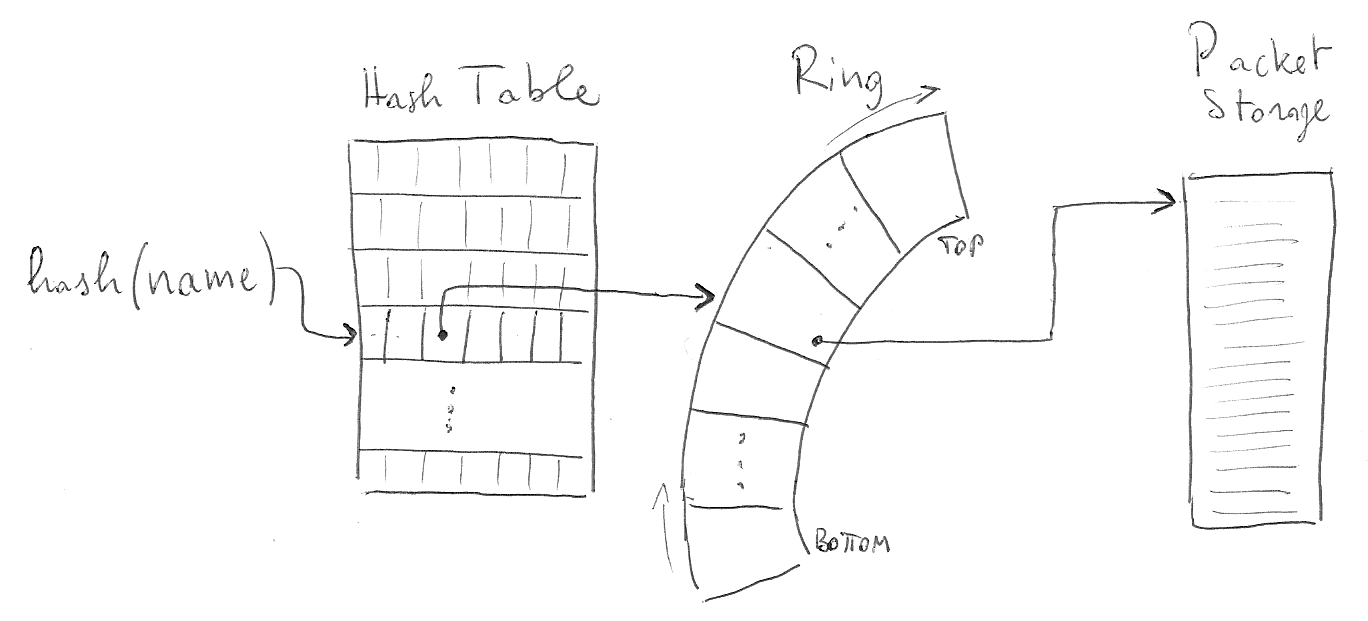
\includegraphics[width=1\textwidth]{img/cs_pit_sketch.png}}
    \caption[Sketch for the data structure for the CS and orignal PIT.]{Sketch of the data structure for the CS. The original PIT design also used the same layout with a hash table and a ring.}
    \label{fig:augustus.ht_ring}
  \end{center}
\end{figure}

The \gls{CS} holds the data packets that are available locally, implementing the in-network caching layer at the packet granularity. In the implementation, packets' content is never moved from the place where the \gls{DMA} operation placed it, in a memory area managed by the DPDK driver. Instead, the reference counters for the cached packets are increased so that the memory manager will not clean it up at sending time.

As outlined in Section \ref{sec:augustus.ccn}, the CS is always queried for exact matches in the name, so a hash table provides a simple and effective way to index cached structures. Moreover, the original designers chose to keep each hash table entry as small as possible by storing pointers to a ring (implemented as a circular array), which in turn stores the complete metadata and the pointer to the full packet, as depicted in figure \ref{fig:augustus.ht_ring}: this allows them to manage collisions by squeezing seven entries into fixed-sized buckets which can be fit into a single cache line. This architecture brings the number of cache misses per query to two in most cases: one for fetching the bucket and one for fetching the full metadata from the ring.

In order to exploit this structure, the name hash works in two stages: first, a 32-bit \gls{CRC} sum of the name is computed, then the bucket index is obtained as the CRC module the HT size: after fetching the bucket, the full \gls{CRC} is compared to the ones stored in each entry in the matching bucket, until a match is found or the bucket end is reached. This way, the ring entry is only loaded from memory (and the full name is compared) only when the 32 bit hash matches; of course, in case of a collision in the CRC hash, this procedure may cause an extra cache miss.

\begin{figure}[tb]
  \captionsetup{type=lstlisting}
  %\centering
  \begin{sublstlisting}[t]{.5\linewidth}
    %\centering
  \begin{lstlisting}[language=c,escapechar=\%]
struct cs_ht_entry {
 bool busy;
 uint32_t crc;
 uint32_t ring_index;
};

struct cs_ring_entry {
 bool active;
 char full_name[MAX_NAME_LEN];
 struct dpdk_pkt *pkt;
 // index in HT for cleanup
 uint32_t bucket_index;
 uint8_t tab_in_bucket;
};
%
    \end{lstlisting}
    \caption{CS internal fields}\label{lst:augustus.cs}
  \end{sublstlisting}%
  \begin{sublstlisting}[t]{.5\linewidth}
    %\centering
  \begin{lstlisting}[language=c]
struct orig_pit_ht_entry {
 bool busy;
 uint32_t crc;
 uint32_t ring_index;
};
struct orig_pit_ring_entry {
 bool active;
 uint64_t expiry;
 uint64_t nonce_bf;
 char full_name[MAX_NAME_LEN];
 uint64_t interface_bitmask;
 // index in HT for cleanup
 uint32_t bucket_index;
 uint8_t tab_in_bucket;
};
    \end{lstlisting}
    \caption{Original PIT internal fields}\label{lst:augustus.oldpit}
  \end{sublstlisting}
  \caption[CS and original PIT internal data structures fields]{Internal data structures fields for CS and PIT (simplified for clarity and brevity).}\label{lst:augustus.cs_oldpit}
\end{figure}

\subsection{Pending Interest Table}\label{sec:augustus.pit}
As the name suggests, the \gls{PIT} stores information for interests that have not been satisfied yet. This is the key structure for building the reverse path that a data packet will have to travel in order to reach the host requesting for it. Moreover, in case two clients request the same resource at about the same time, the PIT entries will be aggregated, thus building a multicast distribution tree for popular content.
As with the \gls{CS}, the PIT is always queried for exact matches.

Because a pending interest might stay so indefinitely (e.g. if the interest or data are lost upstream due to congestion), PIT entries need an expiry time that accounts for a worst-case round trip time from the router to the upstream resource. Meanwhile, long expiry times require the PIT to grow larger in order to fit all possible pending interests in the worst case.

During the experiments, an expiry time of $1$ second was chosen, as it was considered large enough for country-scale geographical installations (even if probably too tight for intercontinental links). Assuming a throughput of $5.5$ \gls{Mpps} (a little above the one actually measured, as detailed in Chapter \ref{chap:test}), this results in a PIT with $5.5$ millions entries, corresponding to about $500$ MB.

In its original implementation, the PIT layout was identical to the CS, with a stripped-down hash table and a ring storing most of the needed data. It obviously differs in the fields stored in the ring entry, as highlighted in listing \ref{lst:augustus.cs_oldpit}. The remaining parts of this Section highlight the limitations of this approach and introduce an improved design overcoming them.

\subsubsection{PIT purging issue}\label{sec:augustus.pit.purge}
The described approach introduced the need for a PIT purging procedure: while the management of the ring structure is extremely simple and efficient when operated in a FCFS manner (as in the CS), it only allows a contiguous region of cells to be occupied. Thus, whenever a data packet comes that matches an entry other than  the bottom one, it has to be lazily deleted until all ``previous'' entries (i.e. the ones between the bottom pointer and the deleted one) are also deleted.  
Thus, the purging procedure was designed in order to clean up space from the entries at the bottom of the ring that were either expired or lazily deleted.

This procedure proved to work smoothly for the case where all interests were eventually satisfied. However, whenever even a single PIT entry came to expiry, it would prevent the purging procedure to be effective for $1$ second (the expiry time). In the meanwhile, when operating at the maximum rate, almost all the remaining entries would fill up and never get freed, blocked by the one bound to expire. Finally, after the expiration of the blocking entry, the purging procedure would free all the entries marked for deletion, up to the first valid one; at that point, the entries to be cleaned were often in the order of one million, causing the purge procedure to take $10$ to $15$ milliseconds to run: at the rate achieved by the router, this corresponds to about $13000$ to $20000$ packets that would be lost in a row.

\subsubsection{Improved data structure design}\label{sec:augustus.pit.new}

\begin{figure}[tb]
  \begin{center}
    \frame{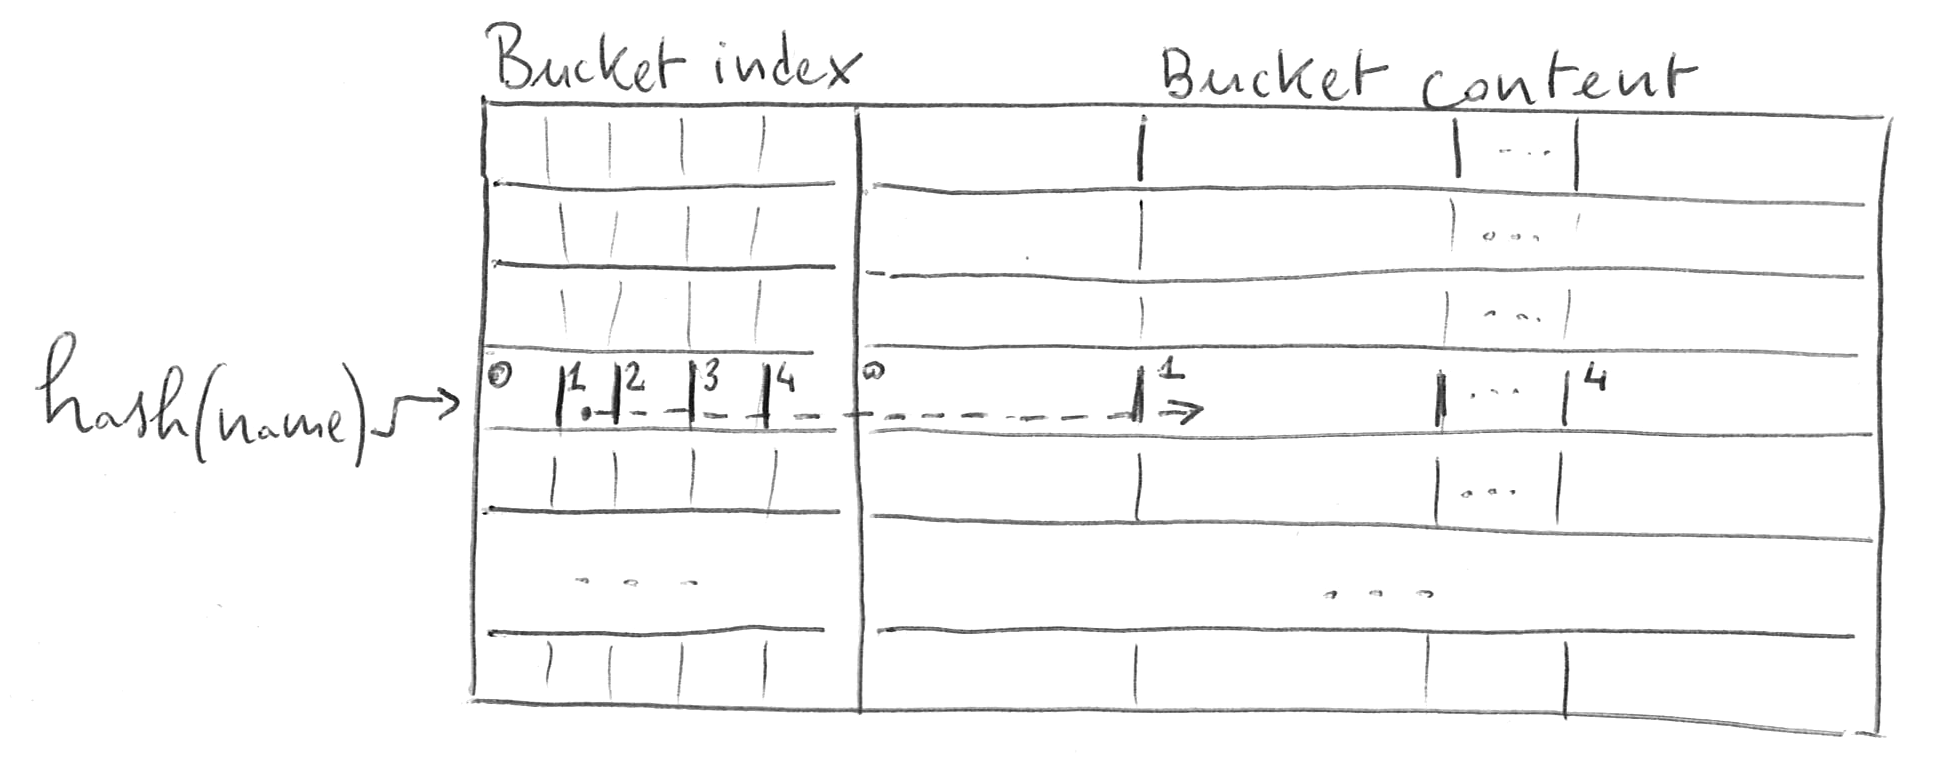
\includegraphics[width=1\textwidth]{img/new_pit_sketch.png}}
    \caption[Sketch for the improved PIT data structure]{Sketch for the improved PIT data structure.}
    \label{fig:augustus.newpit}
  \end{center}
\end{figure}

\begin{figure}[tb]
  \captionsetup{type=lstlisting}
  %\centering
  \begin{sublstlisting}[t]{.5\linewidth}
    %\centering
  \begin{lstlisting}[language=c]
struct pit_index_entry {
 bool busy;
 uint32_t crc;
 uint64_t expiry;
};
struct pit_body_entry {
 uint64_t nonce_bf;
 char full_name[MAX_NAME_LEN];
 uint64_t interface_bitmask;
};
    \end{lstlisting}
    \caption{Improved PIT internal fields}\label{lst:augustus.newpit}
  \end{sublstlisting}%
  \begin{sublstlisting}[t]{.5\linewidth}
    %\centering
  \begin{lstlisting}[language=c]
struct fib_ht_entry {
 bool busy;
 uint32_t crc;
 uint32_t array_index;
};

struct fib_array_entry {
 char full_prefix[MAX_NAME_LEN];
 uint8_t interface_id;
};
    \end{lstlisting}
    \caption{FIB internal fields}\label{lst:augustus.fib}
  \end{sublstlisting}
  \caption[Internal data structures fields for the improved PIT and the FIB]{Internal data structures fields for the improved PIT and the FIB (simplified for clarity and brevity).}\label{lst:augustus.newpit_fib}
\end{figure}

In order to overcome this issue, a new layout for the PIT was designed and implemented into the router: as depicted in figure \ref{fig:augustus.newpit}, the new design relies solely on a hash table. Nevertheless, following the design principle that guided the original development, the first cache line of each bucket is used as an index for the ones to come: as detailed in listing \ref{lst:augustus.newpit}, the bucket index contains the full 32 bit CRC hash, one bit indicating the slot's occupancy and the expiry timestamp. This way, the new structure keeps the property that, except for CRC collisions, a single cache miss is enough to determine whether a name is present as a valid entry in the PIT.

Note that this new structure does not require a periodic purge operation: after loading the bucket index from main memory, the lookup procedure may scan the whole bucket index with no additional memory operations, treating expired entries as empty slots.

Section \ref{sec:test.pit} presents a comparison of the packet loss profile before and after introducing the new PIT implementation.

\subsection{Forwarding Information Base}\label{sec:augustus.fib}
The \gls{FIB} is the structure that, similarly to an IP routing table, holds next-hop information for all known name prefixes and is read-only during data plane routing. Comparing to IP routing tables, however, the \gls{FIB} needs to span a much larger addressing space.

Also the basic part of the FIB structure is similar to the other data structures presented so far, as outlined in listing \ref{lst:augustus.fib}: a stripped-down hash tables with pointers to an external array where the rest of the data is stored. Note that, this time, there is no need for any special management for the external array, as it will be filled sequentially and, as long as the data plane is concerned, entries are never updated nor deleted.

Moreover, the complete implementation of the Augustus router employs an additional \emph{prefix bloom filter} for faster longest prefix lookups: as detailed in the presenting the Caesar router by Perino et al. \cite{caesar}, which provided a starting point for the fully-software reimplementation in Augustus. This structure relies on multiple bloom filters in order to determine (with the possibility of infrequent errors) the length of the prefix that should be looked up in the hash table.
Nevertheless, because this technology was going through the patenting process, the implementation was not disclosed and we could not try it.

Because we could not experiment with its full implementation, the \gls{FIB} was never put under stress throughout the experimental evaluation described in Chapter \ref{chap:test}.

%%%%%%%%%%%%%%%%%%%%%%%%%%%%%%%%%%%%%%%%%%%%%%%%%%%%%%%%%%%%%%%%%%%%%%%%%%%%%%%
\section{Multi-threading and NUMA awareness}\label{sec:augustus.numa}
The Augustus router targets modern servers that are most often equipped with multiple CPU sockets, each containing multiple processing cores. The management of processing cores is aided by the DPDK abstraction library, which natively supports multi-threading and requires to pin at initialization time each thread (called a logical core, or \mono{lcore} in DPDK) to a physical processor: this prevents unneeded context switches, better exploiting local caches.

When multiple CPU sockets are installed on a server, it is common that separate memory banks are directly attached to each one, resulting in a \glsfirst{NUMA} architecture: each processing core has a direct access to memory allocated on a bank on the same socket (called NUMA node), while access to ``remote'' memory is slower and may cause extra bus conflicts.

Moreover, in the context of high-speed packet routing, it is not feasible to manage shared data structures with semaphores, as they introduce an excessive overhead: whenever possible, thread-private data structures are used for read/write operations and shared structures are accessed read-only by all-but-one threads.

In the Augustus router, both the \gls{PIT} and \gls{CS} structures are thread-private and are allocated on the same socket where the thread runs; the \gls{FIB}, instead, is accessed read-only but is nevertheless replicated on each NUMA node, so that local memory access is always possible.
However, separating the \gls{PIT} and \gls{CS} among the threads poses a strong correctness issue: what if a data packet with a name is handled by a different thread than its corresponding interest packet? If this happens, the thread handling the data packet will not find a matching pending interest and will drop the packet as spurious. The same goes for successive interests for the same name, that should result in either a CS hit or in a PIT aggregation.

To overcome this issue, the hardware multiqueue system available in modern NICs is configured to inspect the incoming packets and read a header field holding a hash of the content name, so that it will dispatch packets referring to the same name consistently to the same hardware queue: each queue is polled by a single thread, guaranteeing that two packets with the same name will be delivered to the same thread.

%%%%%%%%%%%%%%%%%%%%%%%%%%%%%%%%%%%%%%%%%%%%%%%%%%%%%%%%%%%%%%%%%%%%%%%%%%%%%%%
\section{Click module port}\label{sec:augustus.click}
\lstinputlisting[float=bt, captionpos=b, label=lst:augustus.click, frame=lines, caption=Sample Click configuration excerpt which uses the API under development]{extra/icnrouter.click.txt}

One limitation posed by the choice of a implementing a standalone software router is that it can not easily coexist on the same hardware (sharing the network cards) with other routing applications. The two main ways to overcome this limitation could be either \begin{inlineenum} \item running the software in a virtual machine, or \item integrating it as a plug-in into an existing routing framework. \end{inlineenum}
While virtualization of network functions is an active research topic and reachable performance could be of the same order of magnitude, the original developers showed a strong interest in porting the router to the \emph{Click} modular router \cite{click}: this approach has the advantage that it builds upon a well established software framework, being able to leverage its most recent ecosystem, ranging from optimized versions (like FastClick \cite{fastclick} or a closed-source version developed at Bell Labs) to the integration with different drivers and even virtualization (through projects like ClickOS \cite{clickos} or NetVM \cite{netvm}).

For these reasons, alongside with the evaluation of the performance of the standalone router implementation described so far and in Chapter \ref{chap:test}, a work was started towards the porting of the router as a Click element library. The porting work is not part of this thesis and is being developed by Raihana Ferdous, a Ph.D. student at the ANS lab, in close collaboration with the original Augustus authors at Bell Labs.
Nevertheless, this effort is worth mentioning here in order to show the direction where the project is moving, and because I contributed designing the API and with minor contributions to the element library itself (namely \mono{ICNInputMux} and \mono{ICNOutputDemux}, described hereafter).

Before detailing the API, it is worth to quickly hint at Click's organization and configuration syntax. A Click router is defined by its configuration file, which represents a directed graph of \emph{elements}: packets travel their way along the graph edges, starting from an input element (which either received from the underlying network driver or generates new packets), until an element either drops it or sends it back to a NIC for forwarding. Each element is instantiated by referencing its full name and possibly specifying its parameters: instantiated elements can be given a name with the double colon syntax \mono{::}. Elements can have any number of input and output numbered \emph{ports}, noted with square brackets at the left (inputs) or right (outputs) of the corresponding element, and ports are connected with each other with left-to-right arrows \mono{->}.

Listing \ref{lst:augustus.click} presents a sample (excerpt of a) Click configuration file which uses the proposed API: the single data structures are exposed as Click elements, each accepting a single input port for both interest and data packets. In this context, some care was needed in order to manage output links: note that the routing procedure is based on the notion of interfaces with point-to-point links, and note that throughout the procedure queries on all three data structures may result in a packet being emitted for sending. To simplify this flow, the extra elements \mono{ICNInputMux} and \mono{ICNOutputDemux} were introduced: the input element takes an arbitrary number of inputs and annotates each packet with the input port, emitting all packets on its single output, so that the core elements may inspect this annotation (both the CS and PIT need this). Core elements wishing to send a packet out will emit it on the proper port (port \mono{[1]} for CS and PIT and the only output port for the FIB) after tagging it with the desired output interface (or interfaces, in case of PIT aggregation): the output element will take care of reading the annotation and sending the packet to its corresponding output port (or ports), which must be wired to the output elements symmetrically with respect to inputs.

The porting work is still ongoing: after my graduation I will probably get more directly involved and, once the development is completed, start working on comparing the performance of the router when running standalone versus as a Click module: while it is likely that a performance penalty will be introduced (due to the added layer of indirection in the software), it will be interesting to find out whether this margin will be low enough to be justified by the increased flexibility.

%%%%%%%%%%%%%%%%%%%%%%%%%%%%%%%%%%%%%%%%%%%%%%%%%%%%%%%%%%%%%%%%%%%%%%%%%%%%%%%
%%%%%%%%%%%%%%%%%%%%%%%%%%%%%%%%%%%%%%%%%%%%%%%%%%%%%%%%%%%%%%%%%%%%%%%%%%%%%%%
%%%%%%%%%%%%%%%%%%%%%%%%%%%%%%%%%%%%%%%%%%%%%%%%%%%%%%%%%%%%%%%%%%%%%%%%%%%%%%%

\chapter{Performance evaluation}
\label{chap:test}

This Chapter presents the results of the performance measurements for the Augustus router: it starts providing an overview of the measurements setup (Section \ref{sec:test.env}), giving the basic definition of throughput used throughput the Chapter (Section \ref{sec:test.overhead}) and detailing the functioning and performance of the traffic generator used for the experiments (Section \ref{sec:test.traffgen}).
Section \ref{sec:test.singlecore} starts the Chapter's core presenting the performance of the router when running as a single thread, while Section \ref{sec:test.multicore} deals with the performance measurements for multi-threaded routing presenting the memory access issues introduced with parallelism.
Finally, Section \ref{sec:test.multicore} presents a comparison of the router loss profile after the introduction of the new PIT design described in Section \ref{sec:augustus.pit}.

%%%%%%%%%%%%%%%%%%%%%%%%%%%%%%%%%%%%%%%%%%%%%%%%%%%%%%%%%%%%%%%%%%%%%%%%%%%%%%%
\section{Testing environment}\label{sec:test.env}
The experimental setup was composed of two twin machines, each equipped with two 10 Gbps Ethernet ports:
table \ref{tab:test.hw} summarises their hardware components.

\begin{table}[tb]
  \begin{center}
    \begin{tabular}{ll}
      \toprule
      %\midrule
      CPUs   & 2 $\times$ Intel(R) Xeon(R) CPU E5-2630 v3 @ 2.40GHz \\
      Memory & 4 $\times$ 16 GB @ 1866 MHz\\
      NICs   & 2 $\times$ Intel 82599ES 10-Gigabit SFI/SFP+ Network Connection \\
             & 2 $\times$ Intel I350 Gigabit Network Connection \\
      \bottomrule
    \end{tabular}
  \end{center}
  %\vspace{-.5cm} % prevents latex from preferring to put this in a blank page
  \caption{Hardware configuration for the two test servers}
  \label{tab:test.hw}
\end{table}

Only the 10 Gbps ports were used for the measurements: corresponding ports in the two machines were connected with passive copper cables attached to the SPF+ ports. On each server, one Gigabit port was used for a management connection, while the remaining port was left unused.

The machines were running Linux 3.16. Following installation recommendation by the DPDK authors, the command line for the kernel provided the allocation of 1 GB huge pages, which were then mounted with the dedicated pseudo-filesystem.%
\footnote{\url{https://www.kernel.org/doc/Documentation/vm/hugetlbpage.txt}}
%\footnote{\url{https://web.archive.org/web/20150906011201/https://www.kernel.org/doc/Documentation/vm/hugetlbpage.txt}}

\begin{figure}[tb]
  \begin{center}
    \frame{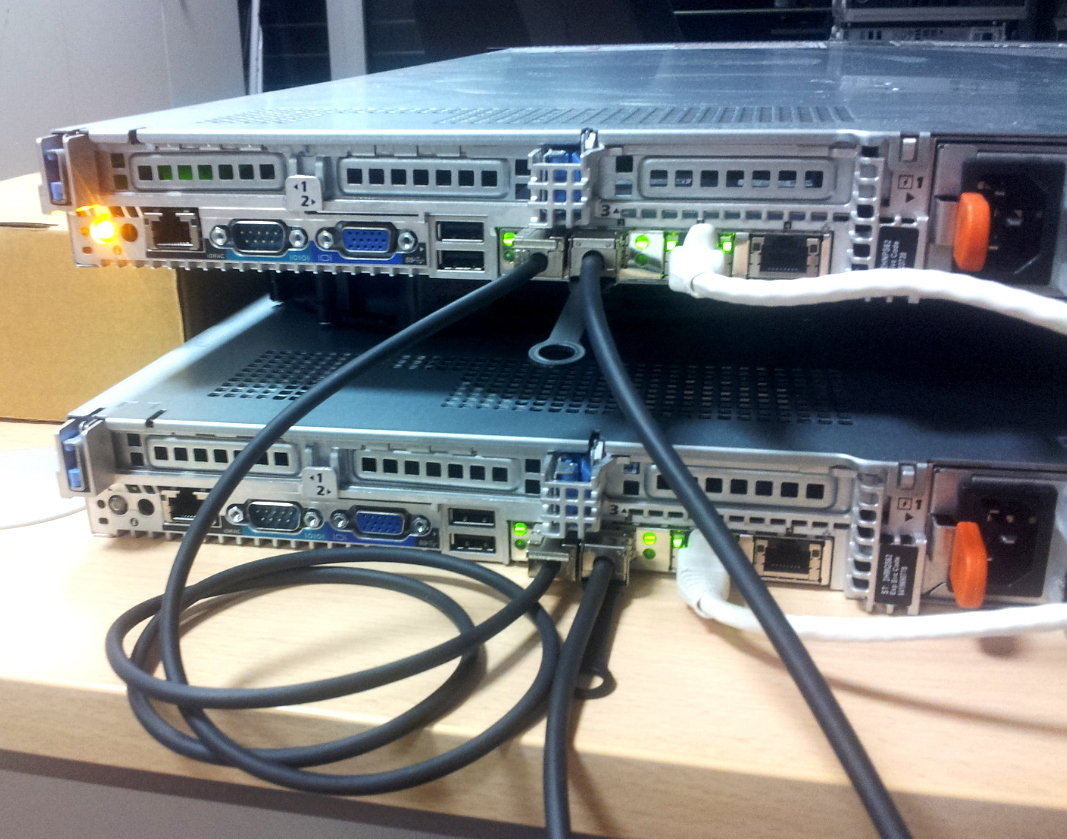
\includegraphics[width=.6\textwidth]{img/servers_back.jpg}}
    \caption[Back panel of the test servers]{Back panel of the test servers, with the SFP+ network ports wired with each other.}
    \label{fig:test.servers_backpane}
  \end{center}
\end{figure}

Of course, this experimental testbed is not the biggest where a tool like Augustus has the potential to be deployed on (indeed, networking devices often cope with tens of full duplex output ports, while we only have two). Nevertheless, the orders of magnitude involved are interesting by themselves, and should still give a rough idea of what we can expect from more powerful deployments.

%%%%%%%%%%%%%%%%%%%%%%%%%%%%%%%%%%%%%%%%%%%%%%%%%%%%%%%%%%%%%%%%%%%%%%%%%%%%%%%
\section{Throughput definition and Ethernet overhead}\label{sec:test.overhead}
Throughout this Chapter, throughput is measured in two main ways: as packet throughput or as bit throughput.
The \emph{packet throughput} is the most straightforward measurement of the routing capabilities of the tested system, and is defined as the number of data packets routed in a given time interval; in most experiments, this means that the actual number of routed packets is at least double, if counting also interest packets.
Defining the \emph{bit throughput} requires the arbitrary choice of the layer where to count bits: here I will use the 802.3 \gls{SDU} layer, defining the bit throughput as the number of L2-payload bits belonging to data packets forwarded per time unit.

This definition has the advantage of being closer to the throughput that would be measured at the application layer. However, this also means that the resulting bit throughput is not directly comparable with the one measured at the physical layer, as reported on NIC data sheets and on physical networking standards.
Indeed, unless the payload is so small that extra padding is required, the transmission of a 802.3 packet adds to the payload at least the equivalent of 38 bytes (octets) on wire \cite{ethernet}:
\begin{itemize}[noitemsep,nolistsep]
\item 7 octets preamble,
\item 1 octet Start of Frame Delimiter,
\item 14 octets header, including the addresses and the type/length field but excluding optional fields like the VLAN tag,
\item 4 octets Frame Check Sequence,
\item Inter-Packet Gap, equivalent to 12 octets.
\end{itemize}
For packets with 46 bytes of L2 payload (which is the minimum size that does not yield any padding in 802.3),the maximum achievable performance over a 10 Gbps link is thus a mere $5.4$ Gbps. Of course, the overhead tends to get smaller for bigger packets and almost negligible for large jumbo frames.

For this reason, throughout the rest of this Chapter all the plots using bit throughput are compared against the maximum throughput achievable at the given packet size.

Every data point presented in the coming Sections was obtained from the router performance at steady state, taking periodic samples and averaging the measure over a time span that ranges from $20$ to $100$ seconds, depending on the variability that was found in the preliminary runs.

%%%%%%%%%%%%%%%%%%%%%%%%%%%%%%%%%%%%%%%%%%%%%%%%%%%%%%%%%%%%%%%%%%%%%%%%%%%%%%%
\section{Traffic generator}\label{sec:test.traffgen}
\begin{figure}[tb]
  \begin{center}
    %\frame{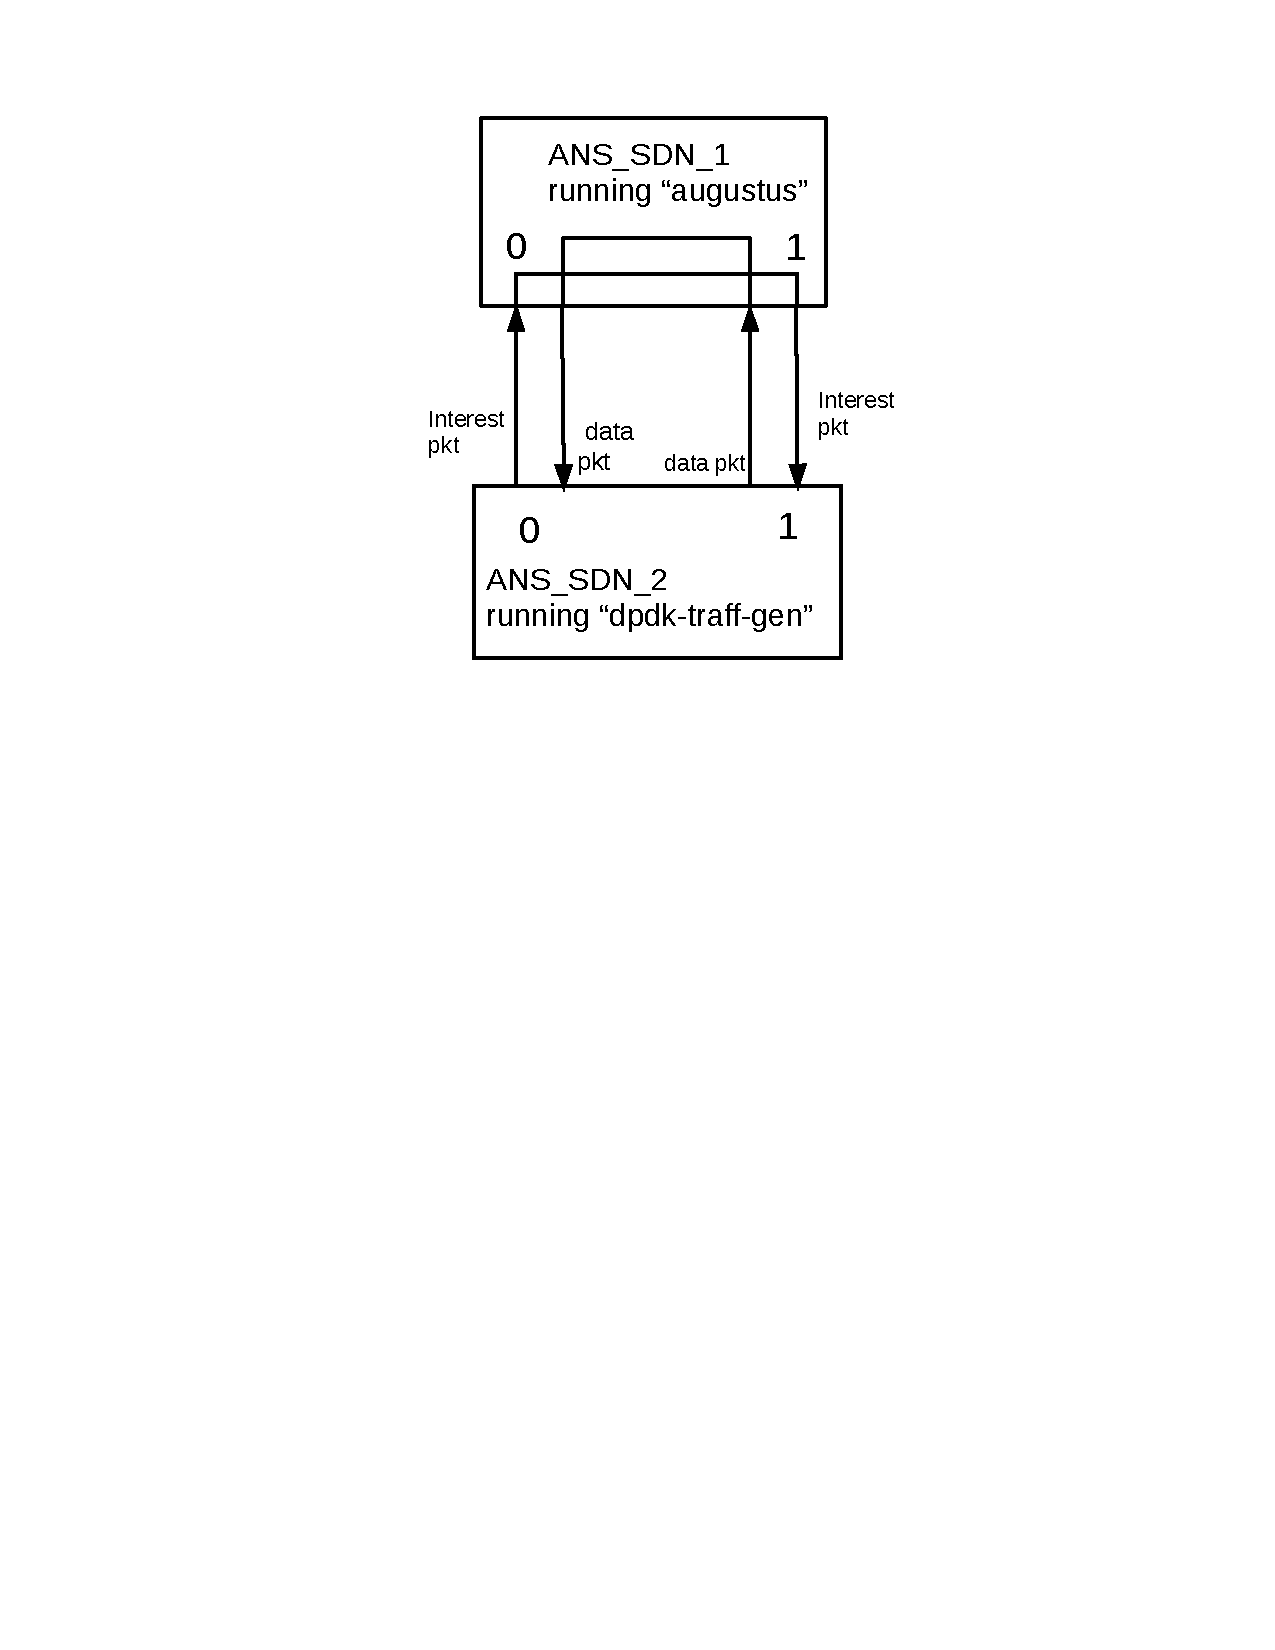
\includegraphics[width=.5\textwidth,draft]{img/test_setup.pdf}}
    \begin{tikzpicture}

  \tikzset{cable/.style={thick}}
  \tikzset{dataline/.style={draw=black!50,ultra thick,->}}
  \tikzset{intline/.style={dashed,draw=black!50,very thick,->}}


  % Basic nodes

  \node [rectangle,draw=black,minimum width=8cm,minimum height=1cm]
    (augustus) {};
  \node [below=1mm of augustus.north] {Augustus Router};
  \node [rectangle,draw=black,minimum width=8cm,minimum height=2cm]
    (pktgen) [below=1.5cm of augustus] {};
  \node [above=0 of pktgen.south] {Traffic generator};
  \node [rectangle,draw=black,minimum width=3cm]
    (intgen) [left=5mm of pktgen.center] {\small Interest generator};
  \node [rectangle,draw=black,minimum width=3cm]
    (echoserver) [right=5mm of pktgen.center] {\small Echo server\vphantom{g}}; % phantom g to align boxes

  % Ports

  \newcommand\port[1]{ \draw #1 +(-3mm,-1pt) rectangle +(3mm,1pt) [fill]}

  \coordinate (augustus p0) at ([xshift=-2cm]augustus.south);
  \coordinate (augustus p1) at ([xshift=2cm]augustus.south);
  \coordinate (pktgen p0) at ([xshift=-2cm]pktgen.north);
  \coordinate (pktgen p1) at ([xshift=2cm]pktgen.north);

  \port{(augustus p0)};
  \port{(augustus p1)};
  \port{(pktgen p0)};
  \port{(pktgen p1)};

  \coordinate (augustus p0 int) at ([xshift=-.2cm]augustus p0);
  \coordinate (augustus p0 data) at ([xshift=.2cm]augustus p0);
  \coordinate (augustus p1 int) at ([xshift=.2cm]augustus p1);
  \coordinate (augustus p1 data) at ([xshift=-.2cm]augustus p1);
  \coordinate (pktgen p0 int) at ([xshift=-.2cm]pktgen p0);
  \coordinate (pktgen p0 data) at ([xshift=.2cm]pktgen p0);
  \coordinate (pktgen p1 int) at ([xshift=.2cm]pktgen p1);
  \coordinate (pktgen p1 data) at ([xshift=-.2cm]pktgen p1);

  % Port-to-port connections

  \node at (augustus p0.north) [anchor=south] {\footnotesize{p0}};
  \node at (augustus p1.north) [anchor=south] {\footnotesize{p1}};
  \node at (pktgen p0.south) [anchor=north] {\footnotesize{p0}};
  \node at (pktgen p1.south) [anchor=north] {\footnotesize{p1}};

  \draw [cable] (augustus p0) -- (pktgen p0);
  \draw [cable] (augustus p1) -- (pktgen p1);

  \draw [intline] (pktgen p0 int) -- (augustus p0 int)
    node [midway, above, sloped] {\footnotesize{interest}};
  \draw [intline] (augustus p1 int) -- (pktgen p1 int)
    node [midway, above, sloped] {\footnotesize{interest}};

  \draw [dataline] (pktgen p1 data) -- (augustus p1 data)
    node [midway, above, sloped] {\footnotesize{data}};
  \draw [dataline] (augustus p0 data) -- (pktgen p0 data)
    node [midway, above, sloped] {\footnotesize{data}};

  % Intra traffic generator connections

  \draw [intline,thin,<-] (pktgen p0 int) -- (pktgen p0 int |- intgen.north);
  \draw [dataline,thin] (pktgen p0 data) -- +(0,-5mm) -| ([xshift=-1.2cm]echoserver.north);
  \draw [intline,thin] (pktgen p1 int) -- (pktgen p1 int |- echoserver.north);
  \draw [dataline,thin,<-] (pktgen p1 data) -- (pktgen p1 data |- echoserver.north);

\end{tikzpicture}

    \caption{Traffic flow for the router evaluation experiments.}
    \label{fig:test.flow}
  \end{center}
\end{figure}
All the measurements described hereafter have been taken with the aid of a custom traffic generator software running on the other server. The traffic generator, initially developed at Alcatel-Lucent Bell Labs together with the router, is also based on DPDK and shares the packet inspection utilities with the main router. While its core was left mostly unchanged, during the measurement campaign it was extended to support all the scenarios described in the next sections.

The traffic generator implements two main functionalities: the \emph{interest generator} initialises a pool of interest packets and sends them at a chosen pace towards one output port; the \emph{echo server}, instead, listens for incoming packets (on either port) and replies to each interest packet with a data packet containing garbage data associated to the requested resource name. The echo server also recognises incoming data packets and keeps records of the number of packets and bytes it receives: these counters constitute the base for the throughput measurements.

Some of the additions developed during the thesis work include support for:
\begin{itemize}[noitemsep,nolistsep]
  \item extended run-time configuration (most parameters were only modifiable at compile-time, which is not practical for running iteratively while tuning a parameter);
  \item per-port throughput counters;
  \item periodic and asynchronous counters printouts;
  \item on-NIC checksum computation;
  \item generation of interest packets as a Poisson process.
\end{itemize}

Except when considering the generator by itself, experiments were run using the flow depicted in figure \ref{fig:test.flow}: the interest generator initiates the loop pushing interest packets to port 0; interest packets then reach the router from port 0, and all names match \gls{FIB} entries that point to port 1 as their next-hop, so the router stores \gls{PIT} entries all pointing to port 0 and forwards all interests to port 1; interests are then received from the echo server and the corresponding data reply is generated and sent back through port 1: the router will then query the \gls{PIT} and forward the data packets through port 0; on the other side, data packets will be received, counted and dropped by the echo server.
 
\subsection{Generation performance}
\begin{figure}[tb]
  \begin{center}
    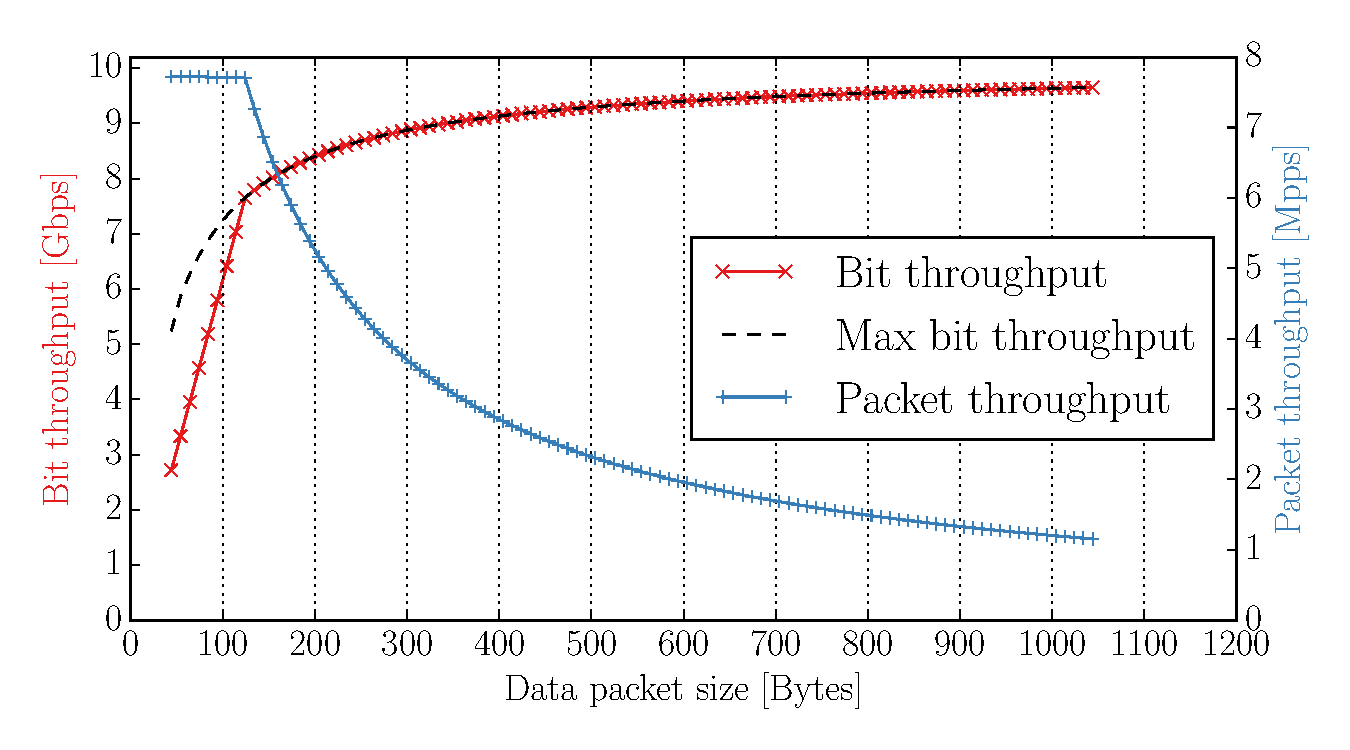
\includegraphics[width=1.0\textwidth]{img/traffgen_increasing_len.pdf}
    \caption[Performance of the traffic generator alone]{Performance of the traffic generator alone. Note that the measurements here were extremely stable, with 3 to 5 significant digits.}
    \label{fig:test.traffgen-perf}
  \end{center}
\end{figure}
Before starting to measure the router performance, it was useful to test the generator by itself in order to have a baseline measure and be sure it was able to fully load the router.
To achieve this, two ports on the same servers were short-circuited together, with the generator running on the machine and sending interest packets on one port: the packets would then be received by the echo server running on the same machine and data would be sent in the backward direction. Finally, the (same) echo server could count the incoming data packets and drop them.

The measurements were taken with one thread running the interest generator and one thread running the echo server, and are shown in figure \ref{fig:test.traffgen-perf}: as expectable, for small packets (up to about 120 bytes) the overall performance is capped by the packet throughput, while for bigger packets the bit throughput limit introduced in Section \ref{sec:test.overhead} is reached.
Because, as highlighted in the coming Sections, this configuration proved to generate enough traffic to load (and overload) the router, the performance using multiple cores were not explored.

\begin{figure}[tb]
  \begin{center}
    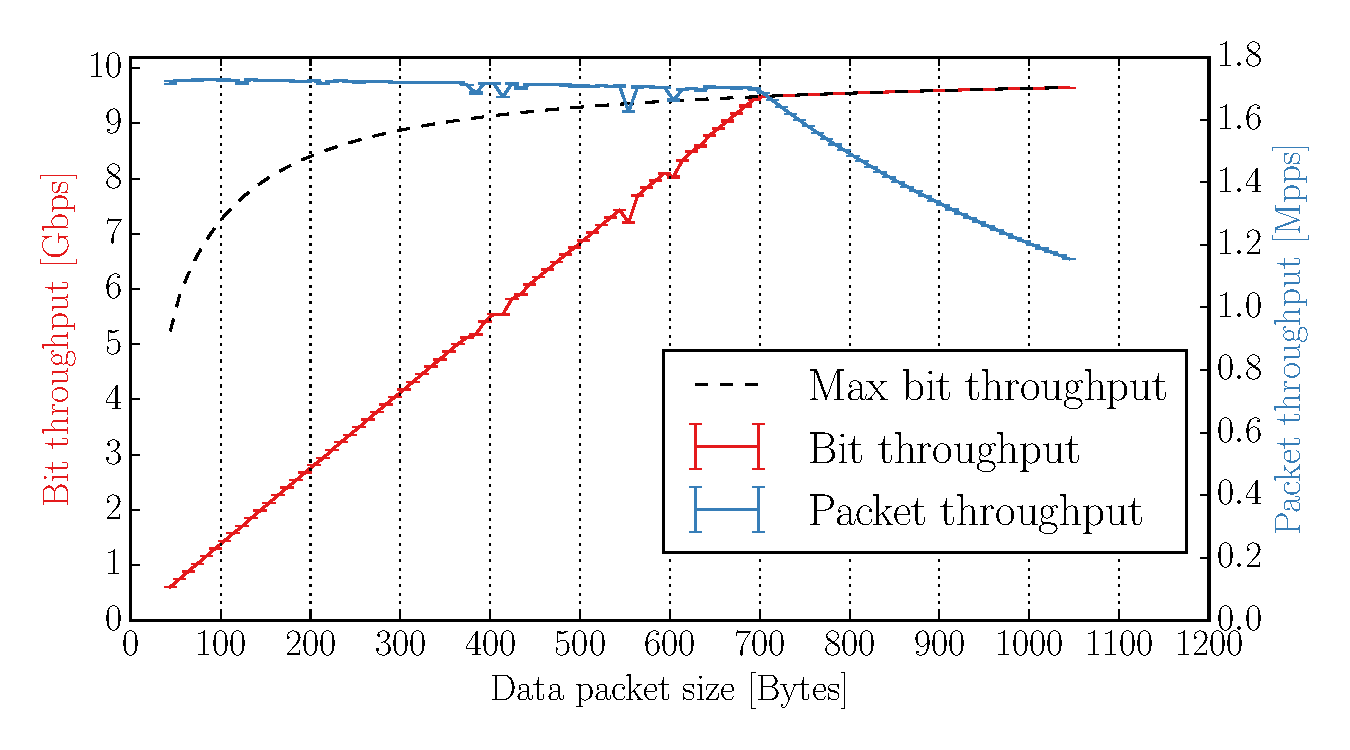
\includegraphics[width=1.0\textwidth]{img/augustus_increasing_len_0x1.pdf}
    \caption[Single-threaded routing performance at varying data packet size]{Routing performance when running the router on a single thread, at varying data packet size.}
    \label{fig:test.incr_len_single}
  \end{center}
\end{figure}
%%%%%%%%%%%%%%%%%%%%%%%%%%%%%%%%%%%%%%%%%%%%%%%%%%%%%%%%%%%%%%%%%%%%%%%%%%%%%%%
\section{Single-threaded routing}\label{sec:test.singlecore}
Figure \ref{fig:test.incr_len_single} presents the performance measured when running the Augustus router in single-thread mode: the maximum packet throughput reached little above $1.7$ \acrfull{Mpps}, with the full bandwidth that is fully exploited for packets starting from 700 bytes. This result is already promising, because in the context of content distribution packets are expected to be fairly large, going as large as the underlying data-link layer supports it when large files are divided into chunks: for example, under Ethernet, packets of up to about 8 kB are supported if jumbo frames are enabled, or else at least 1500 bytes.

%%%%%%%%%%%%%%%%%%%%%%%%%%%%%%%%%%%%%%%%%%%%%%%%%%%%%%%%%%%%%%%%%%%%%%%%%%%%%%%
\section{Multi-threaded routing}\label{sec:test.multicore}
%\begin{figure}[tb]
%  \begin{center}
%    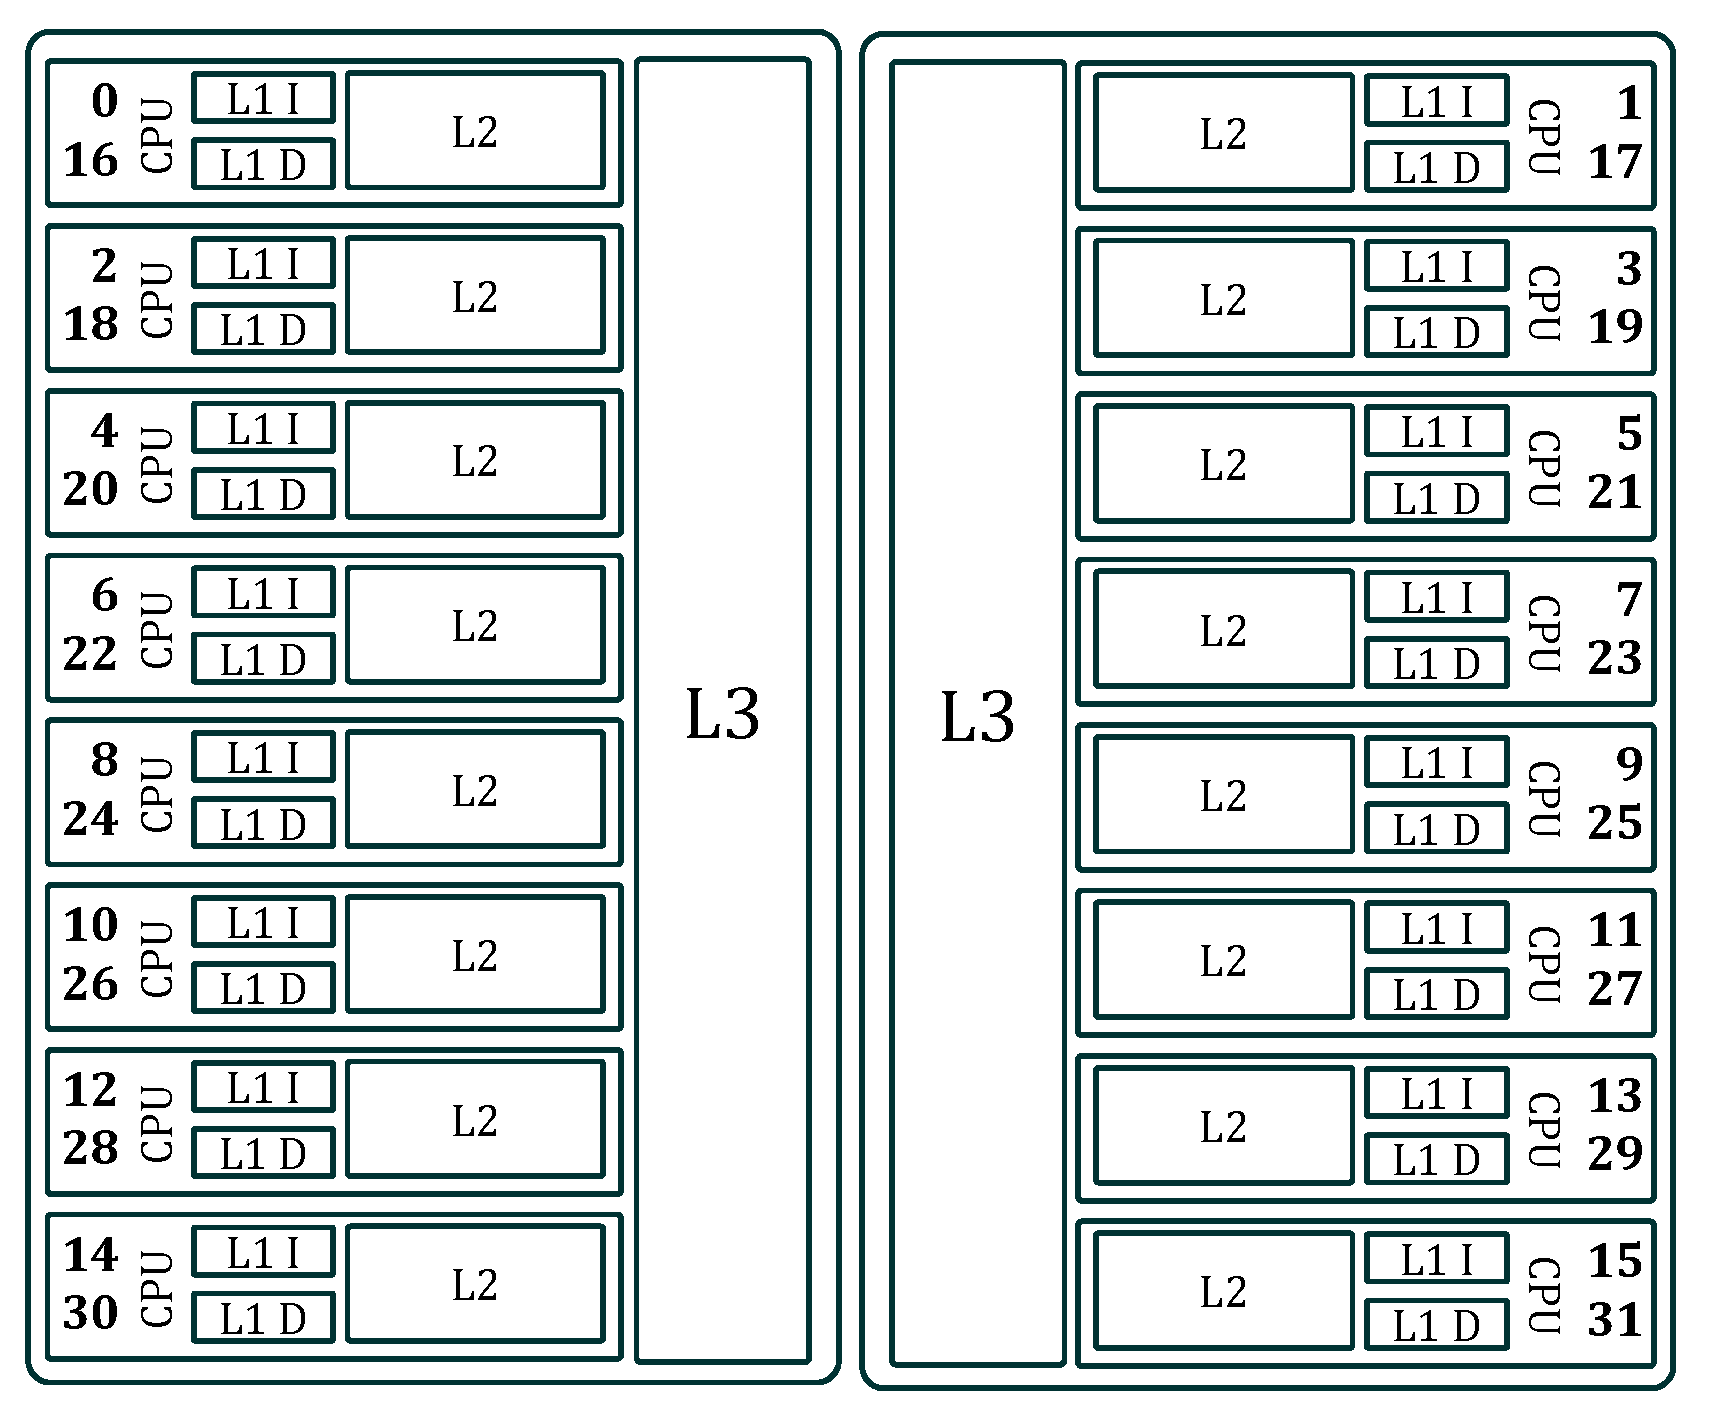
\includegraphics[width=.7\textwidth]{img/cpus_horiz.pdf}
%    \caption[Processors and caches layout on the test servers]{Representation of the processors and caches %layout on the test servers.}
%    \label{fig:test.multicore.cpus}
%  \end{center}
%\end{figure}

Given that, with the precautions described in Section \ref{sec:augustus.numa}, the load can be split among independent workers, multi-threading can be expected to improve on the single-threaded results. However, the amount of performance increase when running multiple threads is non-trivial to tell a priori and, because the routing load is heavily memory-intensive, can not be described as a function of the number of threads alone. This Section first introduces the cache layout of the machines used for the experiments (\ref{sec:test.multicore.layout}), then presents the results of running the router with different number of threads and different thread-to-core mappings (\ref{sec:test.multicore.performance}).

% 2 independently-numbered figures inside a single float by using minipage instead of subfigure
\begin{figure}[t!]
  \centering
  \begin{minipage}{\textwidth}
    \centering
    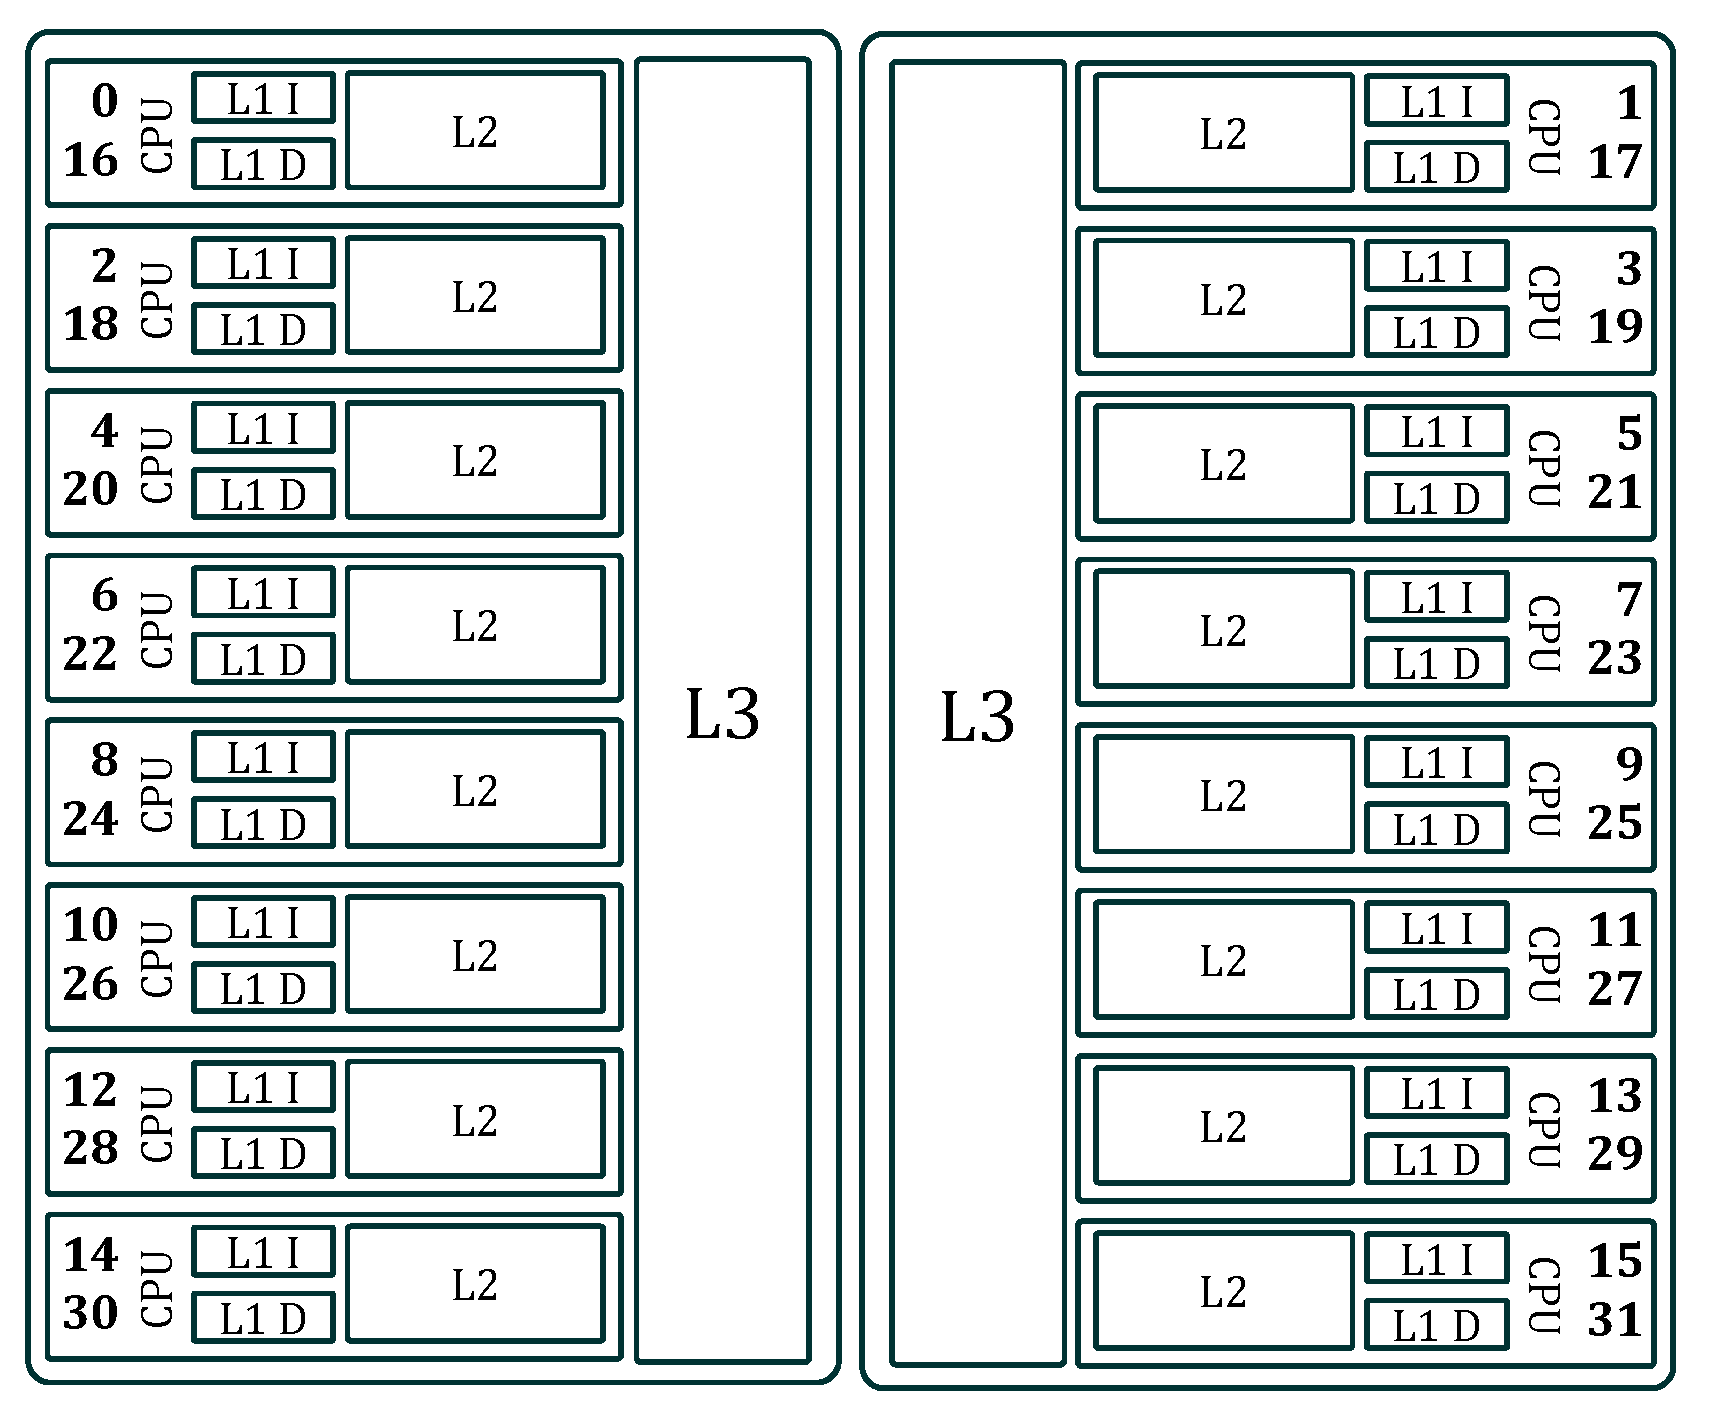
\includegraphics[width=.7\textwidth]{img/cpus_horiz.pdf}
    \caption[Processors and caches layout on the test servers]{Representation of the processors and caches layout on the test servers.}
    \label{fig:test.multicore.cpus}
  \end{minipage}
  \begin{minipage}{\textwidth}
    \centering
    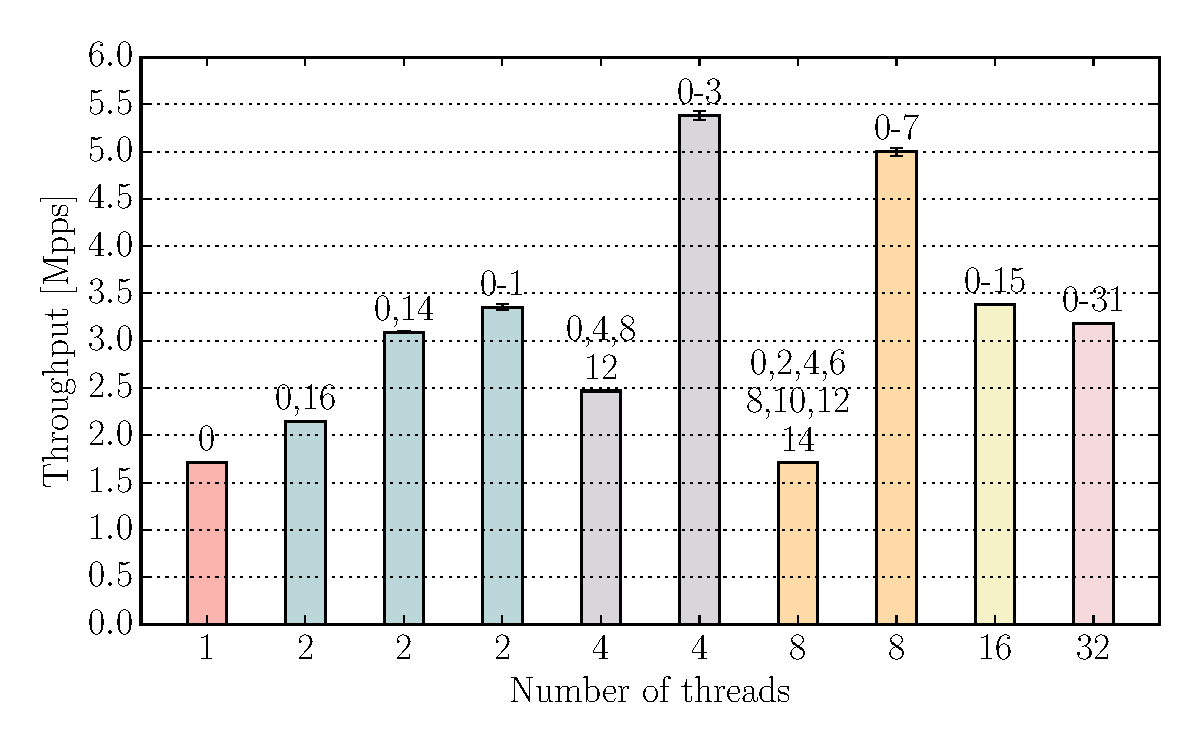
\includegraphics[width=.85\textwidth]{img/augustus_multithread.pdf}
    \caption[Routing performance with different threads count and core pinning]{Routing performance with different threads count and core pinning configurations. The core ID numbers refer to the ones detailed figure \ref{fig:test.multicore.cpus}. These measurements were taken with packets of $94$ bytes.}
    \label{fig:test.multicore.coremap}
  \end{minipage}
\end{figure}

\subsection{CPUs and memory layout}\label{sec:test.multicore.layout}
As anticipated in Chapter \ref{chap:augustus}, the access to the routing data structures makes most of the burden in the routing effort, and cache space is a key resource. Figure \ref{fig:test.multicore.cpus} represents the CPUs and cache layout for the test servers: the two biggest rectangles represent the distinct processor boards installed: each holds $8$ processing cores and each core supports two hardware threads via hyperthreading, for a total of 32 cores as seen by the operating system.
Each socket has a single L3 cache of $20$ MiB, while both L2 and L1 are core-private: each L2 cache holds $2$ MiB while L1 caches hold $512$ KiB each.

\subsection{Performance by core mapping}\label{sec:test.multicore.performance}
%\begin{figure}[tb]
%  \begin{center}
%    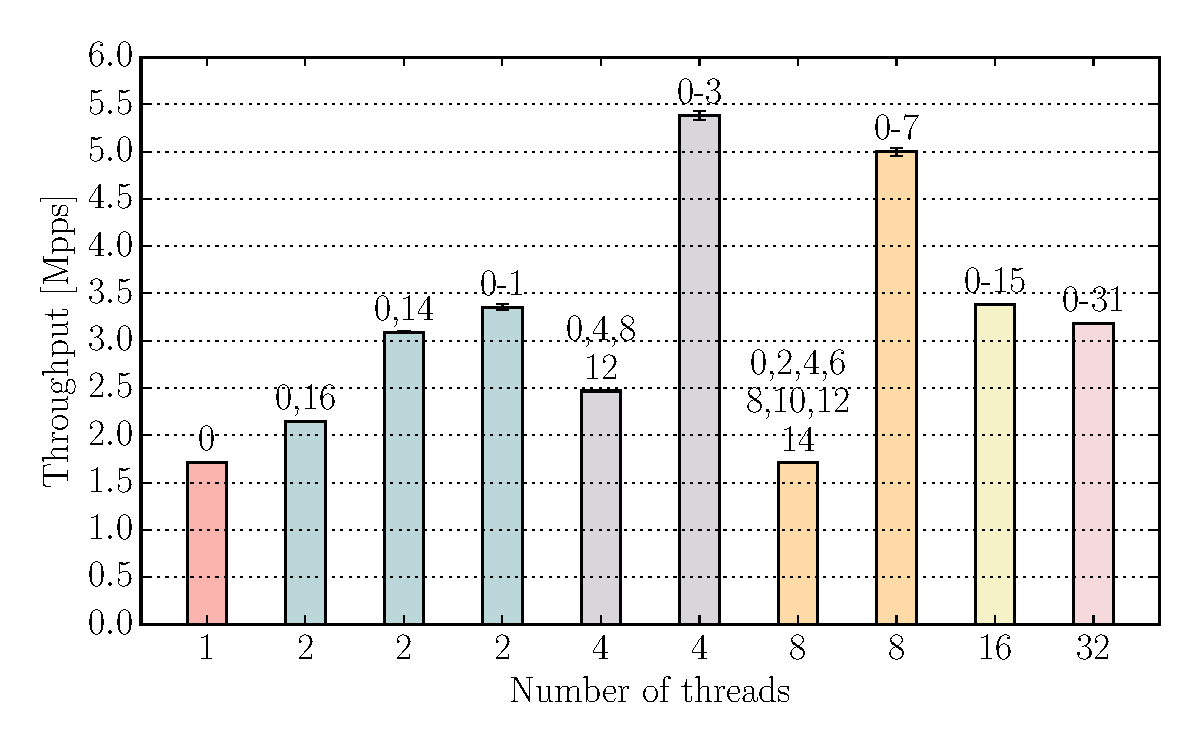
\includegraphics[width=.85\textwidth]{img/augustus_multithread.pdf}
%    \caption[Routing performance with different threads count and core pinning]{Routing performance with different threads count and core pinning configurations. The core ID numbers refer to the ones in figure \ref{fig:test.multicore.cpus}. These measurements were taken with packets of $94$ bytes.}
%    \label{fig:test.multicore.coremap}
%  \end{center}
%\end{figure}

The performance measurements obtained by using different core mappings are shown in figure \ref{fig:test.multicore.coremap}. The first column, at about $1.6$ Mpps, refers to the single-thread execution and repeats the result shown in figure \ref{fig:test.incr_len_single}. The next columns provide results with two threads: running on the two hardware threads on the same core shows a little improvement, which hints that the processing power was probably being the bottleneck in the single-core case. Nevertheless, when using two different cores on the same socket the performance boost from the single thread is little less than doubled, showing that the availability of more L1 and L2 caches does make a difference; finally, in the case where one core per socket is used, performance is actually doubled: this is no surprise, as we have actually doubled the amount of cache and we are now taking full advantage of the NUMA architecture, with L3 cache and CPU-memory buses dedicated to each thread.

Now focus on to the cases with four threads: when placing them on a single socket (``$0,4,8,12$''), even if we are increasing the overall L1 and L2 space, performance are even worse than the homologous 2-threaded case (the column labelled ``$0,14$''): this shows that the bottleneck is now at the level of L3 cache or local memory bus, so adding cores only increases conflicts, with a disastrous result. Moving to the column labelled ``$0-3$'', instead, we can see a $60\%$ improvement, suggesting that one thread per socket was still not fully exploiting the two L3 caches; however, the fact that this improvement is still far from the $2\times$ we got when going from single to dual threads suggests that we hit the limit of either L3 cache or for the access to local memory. Indeed, when trying with 8 processing cores the situation only gets worse, showing that the four cores were able to saturate the I/O capabilities. Finally, continuing to increase the number of threads to $8$, $16$ (one per physical core) or $32$ (one per hardware thread), the situation only gets worse.

\begin{figure}[tb]
  \begin{center}
    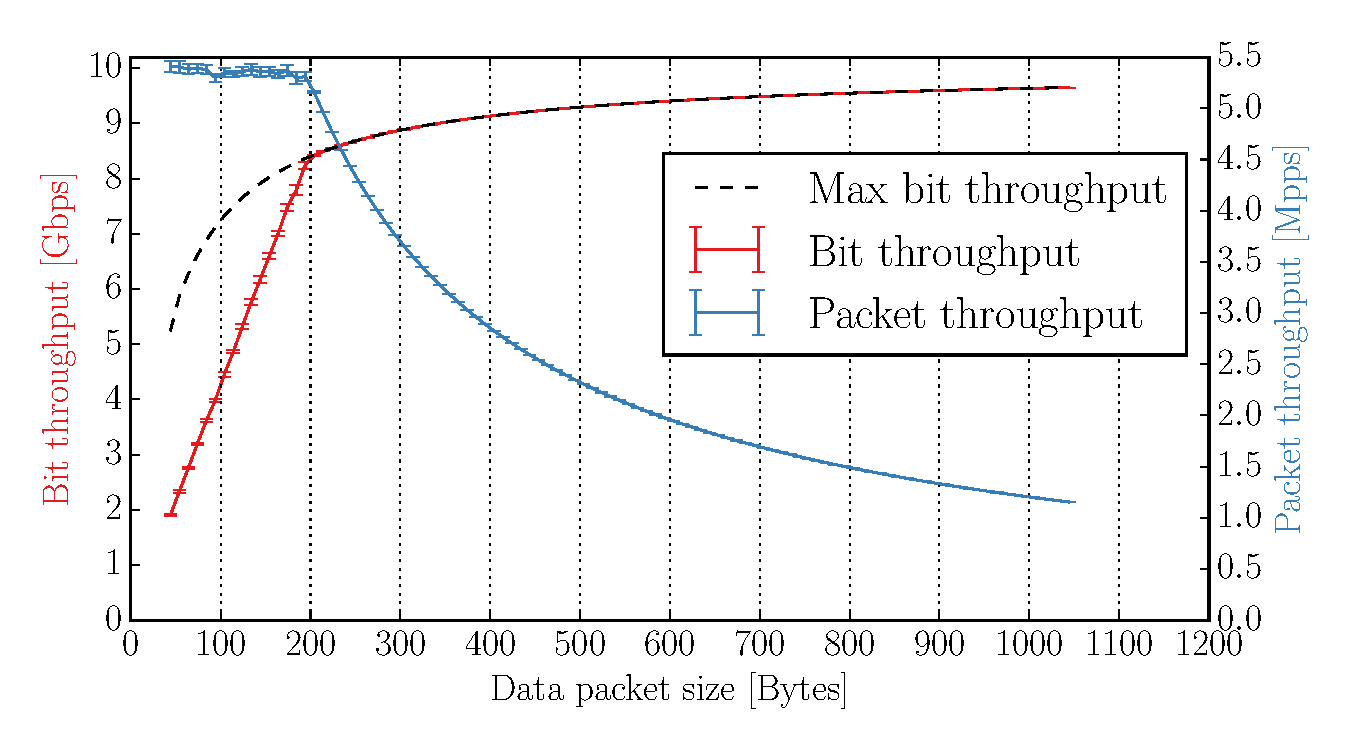
\includegraphics[width=1.0\textwidth]{img/augustus_increasing_len_0xF.pdf}
    \caption[Routing performance at varying data packet for the best multithread configuration.]{Routing performance at varying data packet size using cores 0 through 3, which was found to perform best in the fixed-size measurements outlined in figure \ref{fig:test.multicore.coremap}.}
    \label{fig:test.multicore.incr_len}
  \end{center}
\end{figure}

Figure \ref{fig:test.multicore.incr_len} concludes this measurements showing the throughput profile over packet size for the configuration that performed best in the previous experiment: full line rate exploitation is now reached for packets of 200 bytes already.

%%%%%%%%%%%%%%%%%%%%%%%%%%%%%%%%%%%%%%%%%%%%%%%%%%%%%%%%%%%%%%%%%%%%%%%%%%%%%%%
\section{Evaluation of the new PIT design}\label{sec:test.pit}
While introducing the new implementation for the \acrlong{PIT} described in section \ref{sec:augustus.pit}, it was important to ensure this was actually providing an improvement over the previous one.

\begin{figure}[tb]
  \centering
  \begin{subfigure}[t]{.35\textwidth}
    \centering
    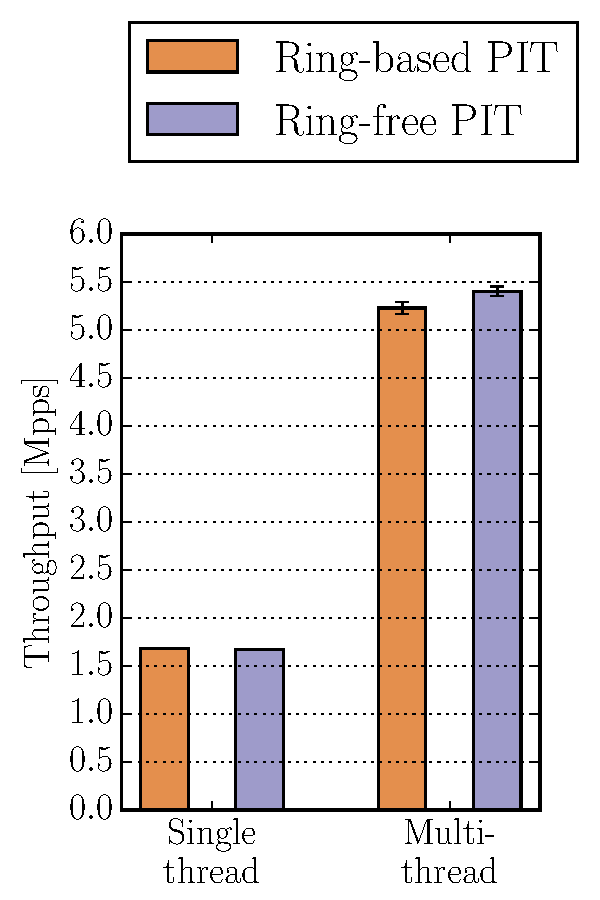
\includegraphics[width=\textwidth]{img/pit_thr_cmp.pdf}
    \caption[]{Overall throughput comparison when introducing the new PIT implementation.}
    \label{fig:test.pit.thr}
  \end{subfigure}
  \unskip ~~
  \begin{subfigure}[t]{.6\textwidth}
    \centering
    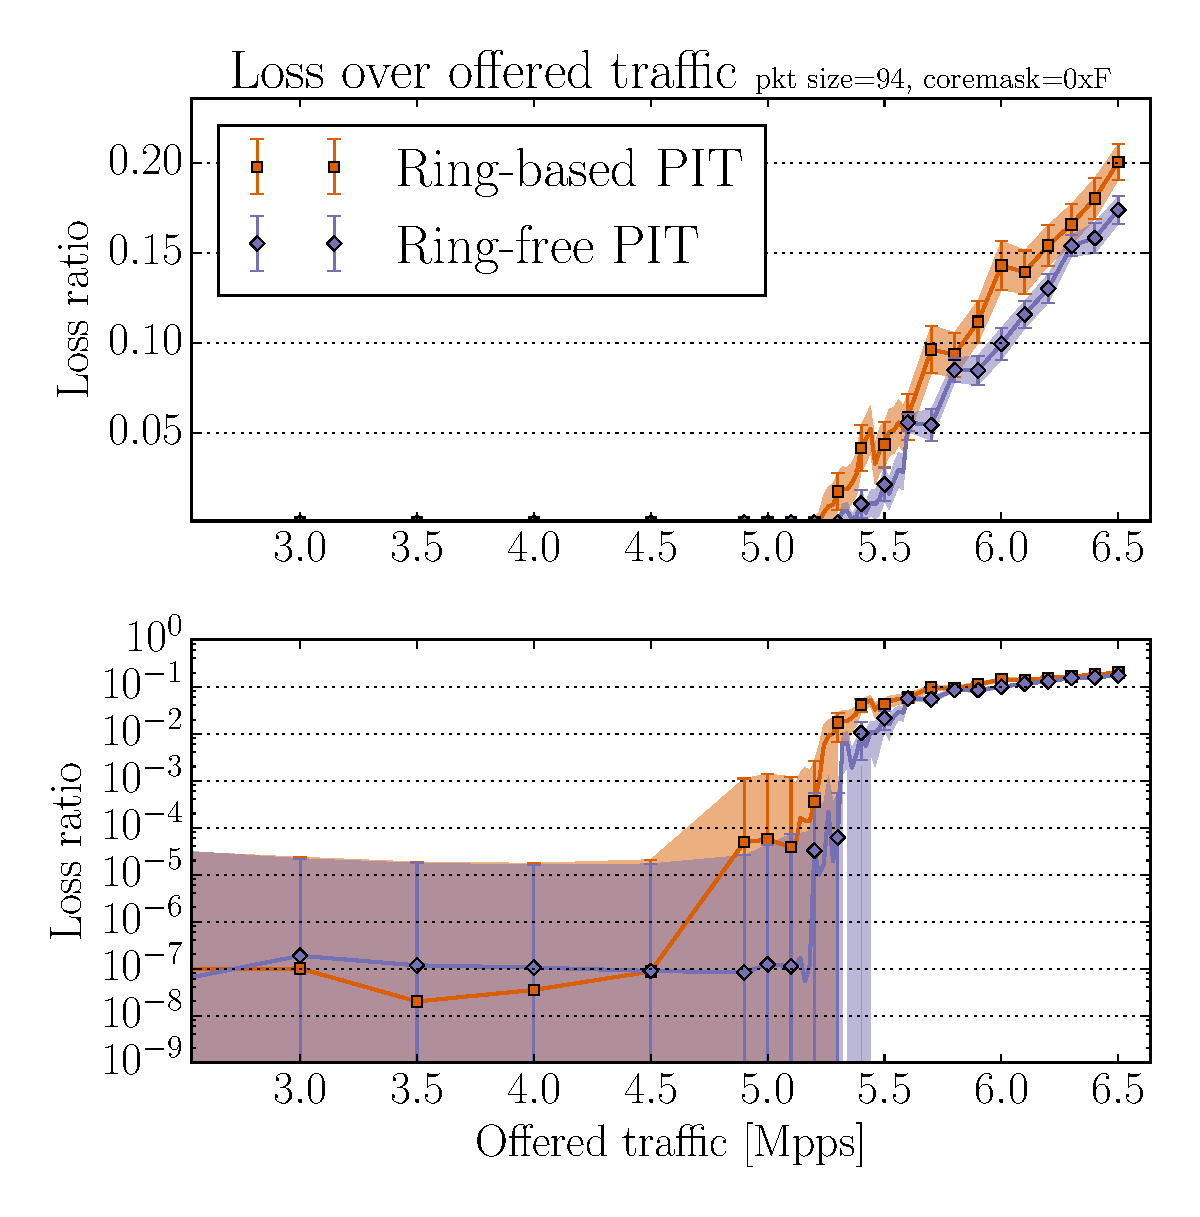
\includegraphics[width=\textwidth]{img/augustus_load_loss.pdf}
    \caption[Effect of the introduction of the new PIT design on the router behaviour in the loss domain]{Effect of the introduction of the new PIT design on the router behaviour in the loss domain. Note that these loss measurements are not precise at all below about $10^{-6}$, resulting in noisy data on the log-scale plot when loss is very close to zero.}
    \label{fig:test.pit.load_loss}
  \end{subfigure}
  \caption[Comparison of the PIT implementations]{Performance comparison of the two PIT implementations.}
\end{figure}
\begin{figure}[tb]
  \begin{center}
  \end{center}
\end{figure}

As a first result, figure \ref{fig:test.pit.thr} \todo{figura superflua?} compares the routing throughput for the different PIT designs for the single-threaded case and for the best multi-threaded case: while the goal of the improved design was not performance improvement at the throughput level, it it interesting to notice that there was no performance penalty either, with even a small improvement in the 4-threaded case (measured under slight overload condition, as measures in previous sections).

\todo[inline]{magari si vedrebbe ancora meglio se l'echo server perdesse dei pacchetti a caso (tipo, in media due al secondo)}
Indeed, as described more in detail in Section \ref{sec:augustus.pit}, the issue with the former design (and the reason it has been replaced) was due to the synchronous purging procedure: whenever a packet was lost and its \gls{PIT} entry came to expiry, it would take tens of milliseconds to purge the space, causing losses in the meanwhile. In our basic evaluation conditions, this happens when offered traffic is close to the maximum achievable throughput. Figure \ref{fig:test.pit.load_loss} shows the loss profile at increasing offered traffic, comparing the behaviour of the router when using the two different designs: it can be seen that the loss for the ring-based PIT starts increasing when the offered load is still lower than its routing capabilities; using the improved (ring-free) PIT, instead, the loss stays close to zero longer, increasing when the offered traffic is close to the maximum routing capacity. Close to the overload condition (from 4.9 to 5.3 Mpps), a loss decrease of over one order of magnitude can be observed.

%%%%%%%%%%%%%%%%%%%%%%%%%%%%%%%%%%%%%%%%%%%%%%%%%%%%%%%%%%%%%%%%%%%%%%%%%%%%%%%
%%%%%%%%%%%%%%%%%%%%%%%%%%%%%%%%%%%%%%%%%%%%%%%%%%%%%%%%%%%%%%%%%%%%%%%%%%%%%%%
%%%%%%%%%%%%%%%%%%%%%%%%%%%%%%%%%%%%%%%%%%%%%%%%%%%%%%%%%%%%%%%%%%%%%%%%%%%%%%%


\chapter{Conclusions}
\label{chap:conclusions}

This work presented a performance evaluation for Augustus, a software implementation of a routing application for \glsfirst{CCN}, focusing only on data plane routing: the software was tested on a general-purpose Linux server equipped with two 10 Gbps Ethernet ports.
The experiments were aided by a custom traffic generation application running on a twin server, which was expanded throughout my work in order to support the required testing scenarios. 
Moreover, during the tests an issue arose with the management and clean-up of the PIT, the data structure that holds the router's soft state in the form of pending interests. A new design was proposed and implemented following the same design principles: the benefits introduced by the new approach were measured, highlighting a decrease in the packet loss of over one order of magnitude when using the new data structure under heavy load conditions.

When running single-threaded, the application managed to route $1.7$ millions of data packets per second, saturating the link with packets of $700$ bytes or larger. Various tests with different multi-threading levels and configurations confirmed the working assumption that the main bottleneck resides in access to main memory, even when using data structures that are designed to minimize the  memory operations by explicit handling of cache-aligned substructures. On the testing environment, the best multi-threaded configuration was reached with four threads running on physical processors distributed among the two \gls{NUMA} nodes, an it yielded $5.4$ millions of data packets per second, saturating the link with packets of just $200$ bytes.

These results are promising in that they show that software defined networking can achieve performance that are ready for medium-scale deployments, even with the load imposed by a \gls{CCN} router, with big data structures that are accessed read/write at the data plane.


%%%%%%%%%%%%%%%%%%%%%%%%%%%%%%%%%%%%%%%%%%%%%%%%%%%%%%%%%%%%%%%%%%%%%%%%%%%%%%%
\section{Future work}\label{sec:future-work}
This work presents a number of limitations and opens the path for future work in many directions. Concerning the performance measurement itself, the results so far are yet missing some relevant considerations:
\begin{itemize}
  \item the experimental evaluation was limited to using the links in a ``prevalent'' direction, so even using the available hardware, it could be possible to better exploit the links and put a load similar to a core router (rather than a boundary router with all content upstream and all clients downstream);
  \item so far, all incoming interests matched the same single entry in the FIB: it is crucial to also include measurements that also put stress on the FIB, as a router of this type should be able to scale to at least millions of entries;
  \item throughout the measurements presented in this work, the \emph{CS} was kept up to date but was never actually used, as each generated interest packet would ask for a different resource name: it is important to also study a model of interest arrivals and dimension the CS so as to maximise the probability of a hit while keeping its size manageable.
\end{itemize}

Moreover, as hinted in Section \ref{sec:augustus.click}, the Click integration is about to be completed and knowing how it performs with respect to the standalone version will be of great interest.

On a broader scale, a lot of work is to be done in the direction of defining and experimenting with control-plane protocols for disseminating routing information in \gls{ICN} networks.


%  SIMPLE PICTURE
%\begin{figure}[htb]
%  \begin{center}
%    \frame{\includegraphics[width=.6\textwidth]{img/maps/pinzolo_slopes.pdf}}
%    \caption[Available maps for Pinzolo ski area]{Available maps for Pinzolo ski area.}
%    \label{fig:map-input}
%  \end{center}
%\end{figure}

% CITE
%In order to achieve this, the map was converted to a 0/1 raster map and the algorithm described in \cite{rthin-algorithm} was run on the rasterized map. %, obtaining the map represented in Figure \ref{fig:map-thinned}.


% TEXTTTT (MONO)
%In particular, \texttt{v.to.rast} module was , single empty pixels surrounded by four filled pixels were forced to be filled.
%However, because it doesn't natively handle topology maps, the obtained refined map was imported back to GRASS GIS, where the topology was finalized and explicit nodes were created using \texttt{v.net} with \texttt{operation\,=\allowbreak\,nodes} (accompanied by \texttt{v.db.addtable} and \texttt{v.category} for properly setting up the attribute table), and spatial attributes like length of edges and altitude of nodes were attached to the respective features.

% ALGORITHM
\begin{comment}
\begin{algorithm}[tb]
%\begin{algorithm}[H]
  \DontPrintSemicolon
  \KwIn{$passages$}
  $passages.sort\_by(\lambda p . new~Couple(p.skipass, p.timestamp))$\;
  $prev := null$\;
  \ForEach{$p \in passages$}{
    $is\_descent := \backslash$\;
    \Indp
      $prev \neq null  \wedge  prev.skipass = p.skipass~\backslash \wedge~prev.day = p.day$\;
    \Indm
    \If{$is\_descent$}{
      \tcp{process descent identified by $prev$ and $p$}
    }
    $prev := p$\;
  }
  \caption[Descents identification]{\textsc{Descents identification}}
  \label{algo:descents}
\end{algorithm}
\end{comment}

\begin{comment}
\begin{table}[tb]
  \begin{center}
    \begin{tabular}{lrrrrr}
      \toprule
        \multicolumn{1}{c}{SD pair} &
        \multicolumn{1}{c}{\specialcell[3cm]{Descents\\percentage}} &
        \multicolumn{1}{c}{\specialcell[3cm]{Log-\\normal}} &
        \multicolumn{1}{c}{Gamma} &
        \multicolumn{1}{c}{Beta} &
        \multicolumn{1}{c}{\specialcell[3cm]{Generalized\\gamma}}\\
      \midrule
      \csvreader[%head to column names,
                 head = true,
                 before line = \\,
                 before first line = {},
                ]
                {tables/fitting_quality.csv}{}{\csvlinetotablerow}
      \\\bottomrule
    \end{tabular}
  \end{center}
  \vspace{-.5cm} % prevents latex from prefering to put this in a blank page
  \caption[Travel time fitting quality]{Fitting quality for some common distributions for every valid SD pair, after applying lunch filtering. SD pairs are identified by the node labels in fig, the second column indicates the percentage of descents for that SD pair with respect to total valid descents. Best fitting values for each row are in bold.}
  \label{tab:traffic-lognorm-fitting}
\end{table}
\end{comment}


\begin{comment}
\begin{figure}[hbt]
  \begin{center}
    %\includegraphics[width=\textwidth]{img/traffic/brenta_groups.pdf}
    \begin{tikzpicture}
      \node (hist) {\includegraphics[width=\textwidth]{img/traffic/brenta_groups.pdf}};
      \node (bwplot) at (hist.north east) [anchor=north east,yshift=-.8cm,xshift=-.9cm]
        {\includegraphics[width=.5\textwidth]{img/traffic/brenta_groups_bw.pdf}};
    \end{tikzpicture}
    \caption[Travel times distributions by group type]{Travel times distributions by group type on Brenta slope. Top panel show the travel time histograms for the identified group types, bottom panel shows a zoom of the same plot on low values. In the box, the representation of the same data as a box plot. Gray lines are log-normal best fitting curves. Note that, in this case, last 5 percentiles were removed independently from each group.}
    \label{fig:traveltimes-groups}
  \end{center}
\end{figure}
\end{comment}


%%%%%%%%%%%%%%%%%%%%%%%%%%%%%%%%%%%%%%%%%%%%%%%%%%%%%%%%%%%%%%%%%%%%%%%%%%%%%%%

%\chapter*{Lists}
%\addcontentsline{toc}{chapter}{Lists}

%\listoffigures
%\listoftables
  %  \cleardoublepage
  %\phantomsection
%\addcontentsline{toc}{chapter}{List of Algorithms}
%\listofalgorithms
%\addcontentsline{toc}{chapter}{List of Listings}
%\lstlistoflistings

\bibliography{davide_kirchner_thesis}


%\printindex  % don't know what this is for, was suggested for glossary...
\printglossaries


%%%%%%%%%%%%%%%%%%%%%%%%%%%%%%%%%%%%%%%%%%%%%%%%%%%%%%%%%%%%%%%%%%%%%%%%%%%%%%%
%~\newpage ~\newpage
%\chapter*{Acknowledgements}
%\addcontentsline{toc}{chapter}{Acknowledgements}


\end{document}
